% --------------------------------------------------------------
% This is all preamble stuff that you don't have to worry about.
% Head down to where it says "Start here"
% --------------------------------------------------------------
\documentclass[12pt]{article}
\usepackage[spanish]{babel}
\usepackage[utf8x]{inputenc}
\usepackage{amsmath}
\usepackage{graphicx}
\usepackage[colorinlistoftodos]{todonotes}
\usepackage{color}
\usepackage{subfigure}
\usepackage{enumitem}
\usepackage{algpseudocode}
\providecommand{\abs}[1]{\lvert#1\rvert}
\providecommand{\norm}[1]{\lVert#1\rVert}
\sloppy
\definecolor{lightgray}{gray}{0.5}
\setlength{\parindent}{0pt}
\usepackage[margin=1in]{geometry} 
\usepackage{amsmath,amsthm,amssymb}
 
\newcommand{\N}{\mathbb{N}}
\newcommand{\Z}{\mathbb{Z}}
 
\newenvironment{theorem}[2][Theorem]{\begin{trivlist}
\item[\hskip \labelsep {\bfseries #1}\hskip \labelsep {\bfseries #2.}]}{\end{trivlist}}
\newenvironment{lemma}[2][Lemma]{\begin{trivlist}
\item[\hskip \labelsep {\bfseries #1}\hskip \labelsep {\bfseries #2.}]}{\end{trivlist}}
\newenvironment{exercise}[2][Exercise]{\begin{trivlist}
\item[\hskip \labelsep {\bfseries #1}\hskip \labelsep {\bfseries #2.}]}{\end{trivlist}}
\newenvironment{reflection}[2][Reflection]{\begin{trivlist}
\item[\hskip \labelsep {\bfseries #1}\hskip \labelsep {\bfseries #2.}]}{\end{trivlist}}
\newenvironment{proposition}[2][Proposition]{\begin{trivlist}
\item[\hskip \labelsep {\bfseries #1}\hskip \labelsep {\bfseries #2.}]}{\end{trivlist}}
\newenvironment{corollary}[2][Corollary]{\begin{trivlist}
\item[\hskip \labelsep {\bfseries #1}\hskip \labelsep {\bfseries #2.}]}{\end{trivlist}}
 
\begin{document}
 
% --------------------------------------------------------------
%                         Start here
% --------------------------------------------------------------
 
%\renewcommand{\qedsymbol}{\filledbox}

\title{Trabajo de estatica en \LaTeX}

\author{Beicker Baena Baldiris \and Yeison Sarmiento Lopez \and Yair Franco Puello \and 'Alvaro Polo Ulloque\and\ Dayana Jimenez Perez} 

\begin{titlepage}

\newcommand{\HRule}{\rule{\linewidth}{0.5mm}} % Defines a new command for the horizontal lines, change thickness here

\center % Center everything on the page
 
%----------------------------------------------------------------------------------------
%	HEADING SECTIONS
%----------------------------------------------------------------------------------------

\textsc{\LARGE Universidad Cat\'olica San pablo}\\[1.5cm] % Name of your university/college
\textsc{\Large Matem\'atica para la Computaci\'on}\\[0.5cm] % Major heading such as course name
\textsc{\large }\\[0.5cm] % Minor heading such as course title

%----------------------------------------------------------------------------------------
%	TITLE SECTION
%----------------------------------------------------------------------------------------

\HRule \\[0.4cm]
{ \huge \bfseries Lista de Ejercicios Nro.1 }\\[0.4cm] % Title of your document
\HRule \\[1.5cm]
 
%----------------------------------------------------------------------------------------
%	AUTHOR SECTION
%----------------------------------------------------------------------------------------

\begin{minipage}{0.4\textwidth}
\begin{flushleft} \large
\emph{Entregado por:}\\
Choqueluque Roman David\\Flores Benites, Victor \\Moreno Vera, Felipe Adrian \\Palomino Paucar, Daniel \\Ramos Cooper, Solange Griselly\\% Your name
\end{flushleft}
\end{minipage}
~
\begin{minipage}{0.4\textwidth}
\begin{flushright} \large
\emph{Profesor:} \\
Sergio \textsc{Aquise Escobedo} % Supervisor's Name
\end{flushright}
\end{minipage}\\[2cm]

% If you don't want a supervisor, uncomment the two lines below and remove the section above
%\Large \emph{Author:}\\
%John \textsc{Smith}\\[3cm] % Your name

%----------------------------------------------------------------------------------------
%	DATE SECTION
%----------------------------------------------------------------------------------------

{\large \today}\\[2cm] % Date, change the \today to a set date if you want to be precise

\vfill % Fill the rest of the page with whitespace

\end{titlepage}

\newpage

%
% Lista de ejercicios de repaso
% =======================================================================================================
\section{Lista de ejercicios de repaso}

%
% Ejercicio 16
% ............
\noindent \textbf{Ejercicio 16:}

Para la región dada en la Figura 1, la transformación $T(X) = AX$ definida por $A = \left[\begin{array}{cc}
    1 & k \\
    0 & 1 
\end{array}\right]$ para $k > 0$ realiza una compresión si $0<k<1$, o expansión para $k>1$ (trasquila un cuadrado en un paralelogramo) verifique que los vectores dados por los vértices del cuadrado corresponden a los vértices del paralelogramo. Determine si la transformación lineal tiene inversa, en caso de existir, halle dicha transformación y explique el efecto gráfico de la transformación inversa.
\begin{figure}[htbp]
    \centering
    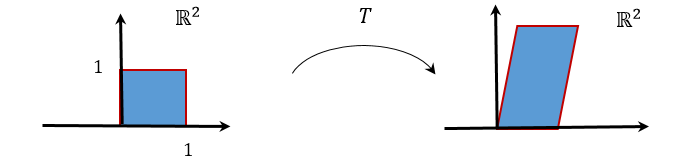
\includegraphics[width=0.8\textwidth]{problema16.png}
\end{figure}

\noindent \textcolor{red}{\bf Solución:}\\

Al aplicar la transformada
\begin{equation}
    T(X) = \left[\begin{array}{cc}
    1 & k \\
    0 & 1 
    \end{array}\right] 
    \left[
    \begin{array}{c}
            x\\
            y\\
    \end{array}
    \right]
\end{equation}
en los vertices del cuadrado se obtiene:
\begin{equation}
    \begin{matrix}
    T\begin{bmatrix}
        0 \\ 
        1
     \end{bmatrix} = \begin{bmatrix}
            k \\ 
            1
       \end{bmatrix} &
    
    T \begin{bmatrix}
        1 \\ 
        1
    \end{bmatrix} = \begin{bmatrix}
        k+1 \\ 
        1
    \end{bmatrix}\\ 
    
    T \begin{bmatrix}
        0 \\ 
        0
    \end{bmatrix} = \begin{bmatrix}
        0 \\ 
        0
    \end{bmatrix} &
    
    T \begin{bmatrix}
        1 \\ 
        0
    \end{bmatrix} = \begin{bmatrix}
        1 \\ 
        0
    \end{bmatrix}\\ 
    \end{matrix}
\end{equation}

\begin{figure}[htbp]
    \centering
    \subfigure[Compresión $0<k<1$]{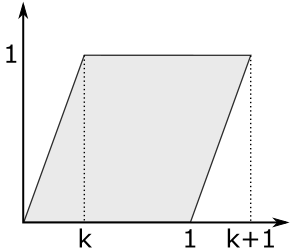
\includegraphics[height=35mm]{paralelogramochiquito.png}}
    \subfigure[Expansión  $1<k$  ]{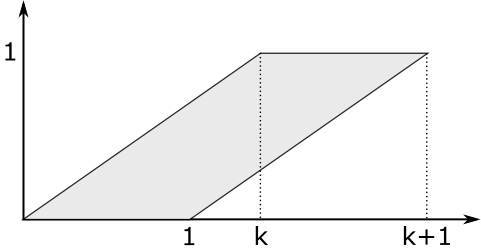
\includegraphics[height=35mm]{paralelogramoalgogrande.png}}
\end{figure}

Para demostrar que la transformación lineal tiene inversa, verificamos que la determinante es diferente de cero:

\begin{equation}
    \left| T \right| =
    \left | \begin{bmatrix}
        1 & k\\ 
        0 & 1
    \end{bmatrix} \right | = 1
\end{equation}
entonces, se demuestra que la transformación lineal es invertible para todo valor de $k$.

%
% Ejercicio 17
% ............
\noindent \textbf{Ejercicio 17:}

Para cada una de las siguientes matrices:\\
$
    a)  
    \begin{bmatrix}
        -1 & 0 \\
         0 & 1
    \end{bmatrix}
    \quad
    b)  
    \begin{bmatrix}
         1 &  0 \\
         0 & -1
    \end{bmatrix}
    \quad
    c)  
    \begin{bmatrix}
         0 & 1 \\
         1 & 0
    \end{bmatrix}
    \quad
    d)  
    \begin{bmatrix}
         \cos{\theta} & -\sin{\theta} \\
         \sin{\theta} &  \cos{\theta}
    \end{bmatrix}
    \quad
    e)
    \begin{bmatrix}
         1 & 0 \\
         k & 1
    \end{bmatrix}
$\\
determine la transformación lineal asociada y en efecto grafico que producirá en la región descrita en
la Figura 2.
\begin{figure}[htbp]
    \centering
    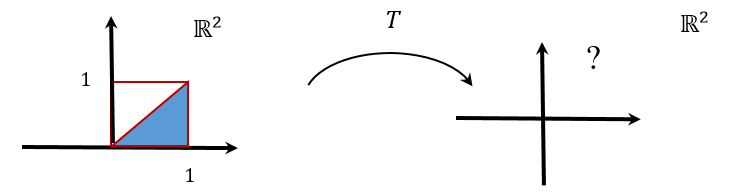
\includegraphics[width=0.8\textwidth]{problema17.png}
\end{figure}

\noindent \textcolor{red}{\bf Solución:}
\begin{enumerate}[label=(\alph*)]

% ....................................................................
\item Dado $T = \begin{bmatrix}
                    -1 & 0 \\
                     0 & 1
                \end{bmatrix}$, aplicamos la transformación lineal a los vértices del triángulo:
    
\begin{equation}
    T \begin{bmatrix}
        0 \\ 
        0
    \end{bmatrix} = \begin{bmatrix}
                        0 \\ 
                        0
                    \end{bmatrix} 
    ,\quad
    T \begin{bmatrix}
        1 \\ 
        1
    \end{bmatrix} = \begin{bmatrix}
                        -1 \\ 
                         1
                    \end{bmatrix}
    ,\quad
    T \begin{bmatrix}
        1 \\ 
        0
    \end{bmatrix} = \begin{bmatrix}
                        -1 \\ 
                         0
                    \end{bmatrix}
\end{equation}

Entonces, el efecto gráfico de la transformación lineal es:

\begin{figure}[htbp]
    \centering
    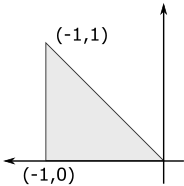
\includegraphics[width=0.18\textwidth]{17a.png}
\end{figure}

% ....................................................................
\item Dado $T = \begin{bmatrix}
                    1 &  0 \\
                    0 & -1
                \end{bmatrix}$, aplicamos la transformación lineal a los vértices del triángulo:

\begin{equation}
    T \begin{bmatrix}
        0 \\ 
        0
    \end{bmatrix} = \begin{bmatrix}
                        0 \\ 
                        0
                    \end{bmatrix} 
    ,\quad
    T \begin{bmatrix}
        1 \\ 
        1
    \end{bmatrix} = \begin{bmatrix}
                         1 \\ 
                        -1
                    \end{bmatrix}
    ,\quad
    T \begin{bmatrix}
        1 \\ 
        0
    \end{bmatrix} = \begin{bmatrix}
                         1 \\ 
                         0
                    \end{bmatrix}
\end{equation}

Entonces, el efecto gráfico de la transformación lineal es:

\begin{figure}[htbp]
    \centering
    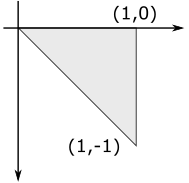
\includegraphics[width=0.18\textwidth]{17b.png}
\end{figure}

% ....................................................................
\item Dado $T = \begin{bmatrix}
                     0 & 1 \\
                     1 & 0
                \end{bmatrix}$, aplicamos la transformación lineal a los vértices del triángulo:

\begin{equation}
    T \begin{bmatrix}
        0 \\ 
        0
    \end{bmatrix} = \begin{bmatrix}
                        0 \\ 
                        0
                    \end{bmatrix} 
    ,\quad
    T \begin{bmatrix}
        1 \\ 
        1
    \end{bmatrix} = \begin{bmatrix}
                        1 \\ 
                        1
                    \end{bmatrix}
    ,\quad
    T \begin{bmatrix}
        1 \\ 
        0
    \end{bmatrix} = \begin{bmatrix}
                        0 \\ 
                        1
                    \end{bmatrix}
\end{equation}

Entonces, el efecto gráfico de la transformación lineal es:

\begin{figure}[htbp]
    \centering
    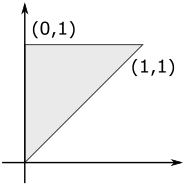
\includegraphics[width=0.18\textwidth]{17c.png}
\end{figure}

% ....................................................................
\item Dado $T = \begin{bmatrix}
                     \cos{\theta} & -\sin{\theta} \\
                     \sin{\theta} &  \cos{\theta}
                \end{bmatrix}$ con $0 \leq \theta \leq 2\pi$, aplicamos la transformación lineal a los vértices del triángulo:


\begin{equation}
    T \begin{bmatrix}
        0 \\ 
        0
    \end{bmatrix} = \begin{bmatrix}
                        0 \\ 
                        0
                    \end{bmatrix} 
    ,\quad
    T \begin{bmatrix}
        1 \\ 
        1
    \end{bmatrix} = \begin{bmatrix}
                        \cos{\theta} - \sin{\theta} \\ 
                        \sin{\theta} + \cos{\theta}
                    \end{bmatrix}
    ,\quad
    T \begin{bmatrix}
        1 \\ 
        0
    \end{bmatrix} = \begin{bmatrix}
                        \cos{\theta} \\ 
                        \sin{\theta}
                    \end{bmatrix}
\end{equation}

Entonces, el efecto gráfico de la transformación lineal es:

\begin{figure}[htbp]
    \centering
    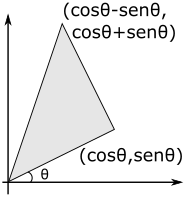
\includegraphics[width=0.18\textwidth]{17e.png}
\end{figure}

Es decir, el efecto gráfico de la transformación lineal es una rotación en $\theta$ grados sobre el origen de coordenadas.

% ....................................................................
\item Dado $T = \begin{bmatrix}
                     1 & 0 \\
                     k & 1
                \end{bmatrix}$ con $k>0$, aplicamos la transformación lineal a los vértices del triángulo:


\begin{equation}
    T \begin{bmatrix}
        0 \\ 
        0
    \end{bmatrix} = \begin{bmatrix}
                        0 \\ 
                        0
                    \end{bmatrix} 
    ,\quad
    T \begin{bmatrix}
        1 \\ 
        1
    \end{bmatrix} = \begin{bmatrix}
                         1 \\ 
                        k+1
                    \end{bmatrix}
    ,\quad
    T \begin{bmatrix}
        1 \\ 
        0
    \end{bmatrix} = \begin{bmatrix}
                        1 \\ 
                        k
                    \end{bmatrix}
\end{equation}

Entonces, el efecto gráfico de la transformación lineal es:\\ \\

\begin{figure}[htbp]
    \centering
    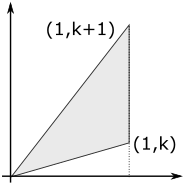
\includegraphics[width=0.18\textwidth]{17d.png}
\end{figure}

\end{enumerate}



%
% Ejercicio 18
% ............
\noindent \textbf{Ejercicio 18:}

Sea $S$ el espacio vectorial de las señales de tiempo discreto. Grafique las siguientes señales $\{y_{k}\}=0.2^{k}$, $\{x_{k}\}=1^{k}$, $\{z_{k}\}=3(-1)^{k}$.\\

\noindent \textcolor{red}{\bf Solución:}\\

Simplificando:\\
$\{x_{k}\}=1$, $\forall k \in Z$\\
$\{y_{k}\}=0.2^{k}$\\
$\{z_{k}\}=3(-1)^{k}$\\

Graficando por planos:\\
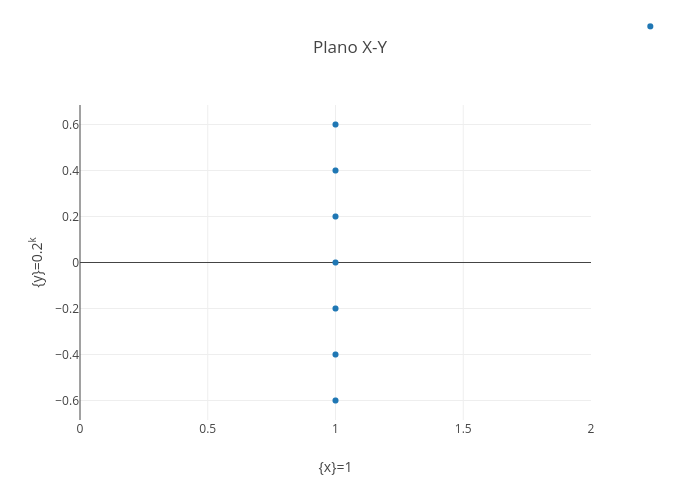
\includegraphics[height=10cm]{PlanoXY.png}\\
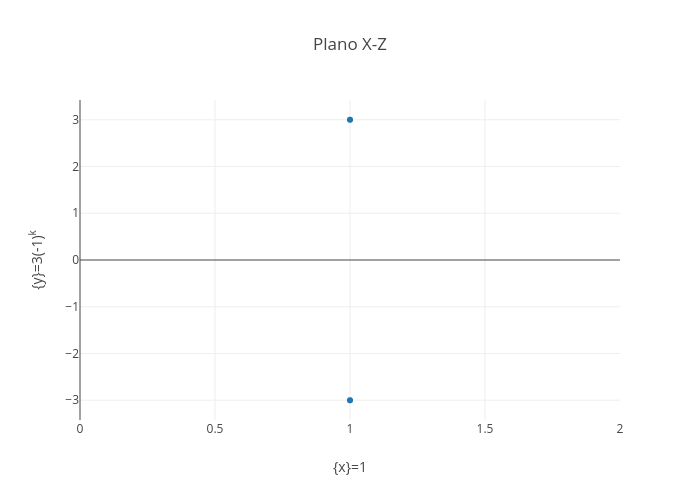
\includegraphics[height=10cm]{PlanoXZ.png}\\
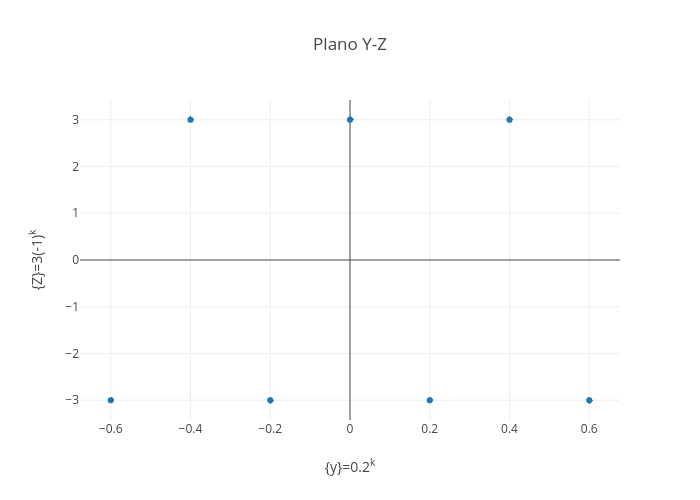
\includegraphics[height=10cm]{PlanoYZ.png}



%
% Ejercicio 19
% ............
\noindent \textbf{Ejercicio 19:}

Verifique que las señales $u_k=1^k$, $v_k=(-2)^k$ , $w_k= 3^k$ son linealmente independientes.\\

\noindent \textcolor{red}{\bf Solución:}\\

Dada la combinación lineal
\begin{equation}
    c_1u_k+c_2v_k+c_3w_k=0
\end{equation}
Suponiendo que la ecuación es cierta para todo $k$, obtenemos:
\begin{equation}
    \begin{matrix}
    c_1u_{k+1}+c_2v_{k+1}+c_3w_{k+1}=0 \\ 
    c_1u_{k+2}+c_2v_{k+2}+c_3w_{k+2}=0
    \end{matrix}
\label{ejer19_1}
\end{equation}
Transformando la Ecuación \ref{ejer19_1} en términos de $c_1, c_2, c_3, w_k$:
\begin{equation}
    \begin{matrix}
    c_1u_k+ c_2v_k+ c_3w_k=0 \\ 
    c_1u_k-2c_2v_k+3c_3w_k=0 \\
    c_1u_k+4c_2v_k+9c_3w_k=0
    \end{matrix}
\end{equation}
Se obtiene la matriz de Casorati:
\begin{equation}
    \begin{bmatrix}
        1 &  1 &  1 \\ 
        1 & -2 &  3 \\ 
        1 &  4 &  9
    \end{bmatrix}
    \begin{bmatrix}
        c_1u_k \\ 
        c_2v_k \\ 
        c_3w_k
    \end{bmatrix} = 
    \begin{bmatrix}
        0 \\ 
        0 \\ 
        0
    \end{bmatrix}
\end{equation}
Las señales $u_k$, $v_k$ , $w_k$ son linealmente independientes si la determinante de la matriz de Casorati es diferente de cero.
\begin{equation}
    \left| \begin{bmatrix}
                1 &  1 &  1 \\ 
                1 & -2 &  3 \\ 
                1 &  4 &  9
           \end{bmatrix} \right| = -30
\end{equation}

Como la determinante es diferente de cero, entonces $c_1=0$, $c_2=0$ y $c_3=0$. Por lo tanto $ \{ u_k, v_k, w_k \}$ son linealmente independientes.\\


%
% Ejercicio 20
% ............
\noindent \textbf{Ejercicio 20}

Dados los escalares $a_0, ..., a_n$ con $a_0$ y $a_n$ distintos de cero y dada una señal $\{z_k\}$, la ecuación definida por:
\begin{center}
$a_0 y_{k+n} + a_1 y_{k+n-1} + ... + a_{n-1} y_{k+1}+a_n y_k = z_k$, $\quad \forall k$
\end{center}
Se denomina ecuación lineal en diferencias o relación lineal de recurrencia de orden n. En el procesamiento digital de señales, una ecuación en diferencias describe un filtro lineal y los coeficientes $a_i$ se denominan coeficientes del filtro. Para el filtro:
\begin{center}
    $0.35 y_{k+2} + 0.5y_{k+1} + 0.35 y_k = z_k $
\end{center}
Usando la señal discreta $\{y_k = \cos(\pi k/4)\}$, para algunos valores de $k \geq 0$ calcule y grafique la señal del filtro $\{z_k\}$.\\

\noindent \textcolor{red}{\bf Solución:}\\

Tabulamos la señal del filtro:

\begin{center}
  \begin{tabular}{ | c | c  c  c | c |}
    \hline
    $k$ & $y_{k}$ & $y_{k+1}$ & $y_{k+1}$ & $0.35y_{k+2}+0.5y_{k+1}+0.33y_{k}$\\
    \hline
    0 & 1        & 0.70711  & 0         & 0.70355   \\
    1 & 0.70711  & 0        & -0.70711  & 0         \\
    2 & 0        & -0.70711 & -1        & -0.70355  \\
    3 & -0.70711 & -1       & -0.70711  & -0.99497  \\
    4 & -1       & -0.70711 & 0         & -0.70355  \\
    5 & -0.70711 & 0        & 0.70711   & 0         \\
    6 & 0        & 0.70711  & 1         & 0.70355   \\
    7 & 0.70711  & 1        & 0.70711   & 0.99497   \\
    8 & 1        & 0.70711  & 0         & 0.70355   \\
    9 & 0.70711  & 0        & -0.70711  & 0         \\
    10 & 0       & -0.70711 & -1        & -0.70355  \\
    \hline
  \end{tabular}
\end{center}

Graficando:

\begin{figure}[htbp]
    \centering
    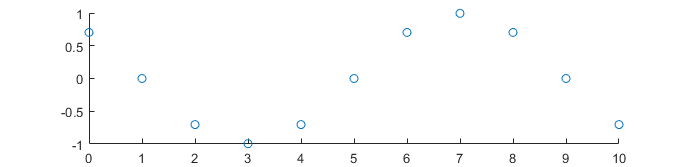
\includegraphics[width=0.9\textwidth]{seno.png}
\end{figure}


%
% Ejercicio 21
% ............
\noindent \textbf{Ejercicio 21:}

Dadas dos funciones $f_1,f_2$ se denomina ortogonales en el intervalo $[a,b]$ si $\int_{a}^{b}f_1(x)f_2(x)dx=0$.
\begin{enumerate}[label=(\alph*)]
    \item Demostrar que el conjunto $\left\lbrace1,\cos{x},\cos{2x},...\right\rbrace$ es ortogonal en el intervalo $[-\pi,\pi]$.
    \item Demostrar que el conjunto $\left\lbrace\frac{1}{\sqrt{2\pi}},\frac{\cos{x}}{\sqrt{\pi}},\frac{\cos{2x}}{\sqrt{\pi}},...\right\rbrace$ es ortonormal en el intervalo $[-\pi,\pi]$.
\end{enumerate}

\noindent \textcolor{red}{\bf Solución:}\\

Realizamos las demostraciones por inducción.

\begin{enumerate}[label=(\alph*)]

    \item Partimos demostrando el caso base: $f_1(x)=1$ y $f_2(x)=\cos{x}$
    \begin{equation}
        \int_{-\pi}^{\pi} \cos{x} dx = sen(\pi)-sen(-\pi)=0
    \end{equation}
    Suponiendo que el conjunto  $\left\lbrace1,\cos{x},\dots,\cos{nx}\right\rbrace$ es ortogonal, demostramos para $\cos{(n+1)x}$:
    \begin{equation}
       \int_{-\pi}^{\pi} \cos{nx}\cos{(n+1)x} dx = \int_{-\pi}^{\pi} \frac{1}{2}\left[ \cos{x}+\cos{(n+1)x} \right] dx
    \end{equation}
    \begin{equation}
       \int_{-\pi}^{\pi} \cos{nx}\cos{(n+1)x} dx  =\frac{1}{2}\left[ \sin{x} + \frac{1}{n+1} \sin{(n+1)x} \right]\bigg\vert_{x=-\pi}^{x=\pi}=0
    \end{equation}
    Por lo tanto, concluimos que el conjunto $\left\lbrace1,\cos{x},\cos{2x},...\right\rbrace$ es ortogonal en el intervalo $[-\pi,\pi]$.

    \item Para que el conjunto sea ortonormal, hacemos que cada función tenga módulo 1. Para el caso base tenemos $f(x)=1/\sqrt{2 \pi }$:
    \begin{equation}
        \left\| f(x) \right\|^2 = \int_{-\pi}^{\pi} (1/\sqrt{2 \pi }) dx = 1/\sqrt{ 2\pi } \int_{-\pi}^{\pi} (1) dx = 1
    \end{equation}
    Para $\cos{nx}$:
    \begin{equation}
        \left\| f(x) \right\| = \sqrt{ \int_{-\pi}^{\pi} \cos{nx}^2 dx } = \sqrt{\frac{1}{2}\int_{-\pi}^{\pi} (1+cos2nx) dx } = \sqrt{\pi}
    \end{equation}
    Por tanto, el conjunto ortonormal es $\left\lbrace\frac{1}{\sqrt{2\pi}},\frac{\cos{x}}{\sqrt{\pi}},\frac{\cos{2x}}{\sqrt{\pi}},...\right\rbrace$.

\end{enumerate}


%
% Ejercicio 22
% ............
\noindent \textbf{Ejercicio 22:}

Si suponemos que $\left \{ \phi _n(x)) \right \}_{ n \in \mathbb{Z} }$, es un conjunto ortogonal infinito de funciones en un intervalo $a \leq x \leq b$. Si $y=f(x)$ es una funcion definida en el intervalo $[a,b]$, es posible determinar los coeficientes $c_n$ para los cuales $f(x)$ se describe como:
\begin{center}
$f(x) = c_0 \phi_0 (x) + c_1 \phi_1 (x) + c_2 \phi_2 (x) + \dots$
\end{center}
a la cual se le denomina Serie de Fourier Generalizada de $f(x)$. Pruebe que sus coeficientes son dados por $c_n=\frac{\int_{a}^{b} f(x) \phi_n (x)  dx }{ \left \| \phi_n (x) \right \|^2 }$.\\

\noindent \textcolor{red}{\bf Solución:}\\

Sea la función: $f(x) = \sum_{k=0}^{\infty} c_k \phi_k (x)$, donde $\left \{ \phi _n(x)) \right \}_{ n \in \mathbb{Z} }$ es un conjunto ortogonal infinito de funciones en un intervalo $a \leq x \leq b$. Se aplica la multiplicación punto entre la funcion $f(x)$ y $\phi_n(x)$, se obtiene:

\begin{equation}
    \left \langle f(x),\phi_n(x) \right \rangle = c_0 \left \langle \phi_0(x),\phi_n(x) \right \rangle 
                                                + c_1 \left \langle \phi_1(x),\phi_n(x) \right \rangle
                                                + \dots
                                                + c_n \left \langle \phi_n(x),\phi_n(x) \right \rangle
                                                + \dots
\end{equation}

Como el producto punto de dos funciones ortogonales es cero, la ecuación queda:
\begin{equation}
    \left \langle f(x),\phi_n(x) \right \rangle = c_n \left \langle \phi_n(x),\phi_n(x) \right \rangle
\end{equation}

Teniendo en cuenta que $\left\| \phi_n (x) \right\| = \sqrt{\left \langle \phi_n(x),\phi_n(x) \right \rangle}$:
\begin{equation}
    \int_{a}^{b} f(x) \phi_n (x)  dx = c_n \left \| \phi_n (x) \right \|^2
\end{equation}

Finalmente:
\begin{equation}
    c_n=\frac{\int_{a}^{b} f(x) \phi_n (x)  dx }{ \left \| \phi_n (x) \right \|^2 }
\end{equation}




%
% Ejercicio 25
% ............
\noindent \textbf{Ejercicio 25:}

Una matriz cuadrada $A = (a_{ij})$ es una matriz banda de amplitud de banda $2k+1$ si $\vert i - j\vert > k$ implica que $a_{ij} = 0$ ¿Cuales son las amplitudes de banda de las matrices tridiagonales y pentadiagonales? ¿es el producto de dos matrices banda con una longitud de banda dada nuevamente una matriz de banda con la misma longitud de banda?

\noindent \textcolor{red}{\bf Solución:}

\begin{enumerate}

\item ¿Cuales son las amplitudes de banda de las matrices tridiagonales?

Una matriz tridiagonal es una matriz cuadrada con elementos distintos a cero en la diagonal principal y las diagonales inmediatamente adyacentes. Es decir, para $\vert i - j\vert > 1$ los elementos $a_{ij} = 0$. La amplitud de banda se define como la cantidad de diagonales diferentes de cero, en el caso de la matriz tridiagonal es igual a $3$.

\item ¿Cuales son las amplitudes de banda de las matrices pentadiagonales?

Una matriz pentadiagonal es una matriz cuadrada con elementos distintos a cero en la diagonal principal y las dos diagonales más cercanas en la parte superior de la matriz, y las dos diagonales más cercanas en la parte inferior de la matriz. Es decir, para $\vert i - j\vert > 2$ los elementos $a_{ij} = 0$. La amplitud de banda de matriz pentadiagonal es $5$.

\item ¿Es el producto de dos matrices banda con una longitud de banda dada nuevamente una matriz de banda con la misma longitud de banda?

Sean las matrices $A = (a_{ij})$, $B = (b_{ij})$, $C = (c_{ij})$ de dimensiones $n \times n$, donde $A$ y $B$ son matrices banda de amplitud de banda $2k+1$ (es decir, para $\vert i - j\vert > k$ los coeficientes $a_{ij}$ son iguales a cero), tal que: $AB = C$.

Analizamos únicamente $c_{0n}$:
\begin{equation}
    c_{0n} = \sum_{p=0}^{n} a_{0p} b_{pn} 
\end{equation}
como $a_{0p} = 0$ para $p>k$ y $b_{p0} = 0$ para $p<k$, tenemos:
\begin{equation}
    c_{0n} = \sum_{p=k}^{k} a_{0p} b_{p0} =  a_{kp} b_{pk}
\end{equation}
como $a_{kp} b_{pk} \neq 0$, entonces la matriz $C$ no es una matrices banda de amplitud $2k+1$.

\end{enumerate}

%
% Ejercicio 26
% ............
\noindent \textbf{Ejercicio 26:}

Pruebe la desigualdad de Schwarz.\\

\noindent \textcolor{red}{\bf Solución:}

La desigualdad de Schwarz es:

\begin{equation}
    \left |\left \langle a,b \right \rangle  \right |^2 \leq \left \langle a,a \right \rangle \left \langle b,b \right \rangle
\end{equation}

En $\mathbb{R}^n$ queda expresado:
\begin{equation}
    \left(\sum _{k=1}^{n}{a_{k}b_{k}}\right)^{2}\leq \left(\sum _{k=1}^{n}{a_{k}^{2}}\right)\left(\sum _{k=1}^{n}{b_{k}^{2}}\right)
\end{equation}
Para demostrar, partimos de la suma de cuadrados:
\begin{equation}
    \sum _{k=1}^{n}{(a_{k}x+b_{k})^{2}}={\Bigl (}\sum _{k=1}^{n}{a_{k}^{2}}{\Bigr )}x^{2}+2{\Bigl (}\sum _{k=1}^{n}{a_{k}b_{k}}{\Bigr )}x+\sum _{k=1}^{n}{b_{k}^{2}}\geq 0
\end{equation}
Esta ecuación es un polinomio cuadrático. Para que el polinomio sea siempre positivo, este debe poseer solo una solución o no debe poseer soluciones reales. Entonces, el discriminante del polinomio debe ser menor o igual a cero.
\begin{equation}
    \Delta =\left(2 \sum _{k=1}^{n}{a_{k}b_{k}} \right)^2 - 4\left( \sum _{k=1}^{n}{a_{k}^{2}} \right)\left( \sum _{k=1}^{n}{b_{k}^{2}} \right)\leq 0
\end{equation}
\begin{equation}
    \left(\sum _{k=1}^{n}{a_{k}b_{k}} \right)^2 - \left( \sum _{k=1}^{n}{a_{k}^{2}} \right)\left( \sum _{k=1}^{n}{b_{k}^{2}} \right)\leq 0
\end{equation}
Finalmente:
\begin{equation}
    \left(\sum _{k=1}^{n}{a_{k}b_{k}} \right)^2 \leq \left( \sum _{k=1}^{n}{a_{k}^{2}} \right)\left( \sum _{k=1}^{n}{b_{k}^{2}} \right) 
\end{equation}

%
% Ejercicio 36
% ............
\noindent \textbf{Ejercicio 36:}

Considerando la matriz de Hilbert de orden n:
$$H_n = \left [ \frac{1}{i+j-1} \right ], 1\leq i, j\leq n $$
\begin{enumerate}[label=(\alph*)]
    \item Determine $H_4$ y muestre que es inversible.
    \item Halle $(H_4)^{-1}$ y use para resolver el sistema $H_4x = b$, donde $b=[2\quad-1\quad3\quad5]^\intercal$
\end{enumerate}


\noindent \textcolor{red}{\bf Solución:}\\

\begin{enumerate}[label=(\alph*)]

\item Matriz de Hilbert $H_4$:
\begin{equation}
    H_4 =   \begin{bmatrix}
                 1  & 1/2 & 1/3 & 1/4 \\ 
                1/2 & 1/3 & 1/4 & 1/5 \\ 
                1/3 & 1/4 & 1/5 & 1/6 \\ 
                1/4 & 1/5 & 1/6 & 1/7
            \end{bmatrix}
\end{equation}
Verificamos que la determinante es diferente de cero:
\begin{equation}
    \left| H_4 \right| = \left|
        \begin{bmatrix}
             1  & 1/2 & 1/3 & 1/4 \\ 
            1/2 & 1/3 & 1/4 & 1/5 \\ 
            1/3 & 1/4 & 1/5 & 1/6 \\ 
            1/4 & 1/5 & 1/6 & 1/7
        \end{bmatrix}
        \right| = 1.653439 \times 10^{-7}
\end{equation}
Se comprueba que la matriz $H_4$ es invertible.

\item La inversa de la Matriz de Hilbert $H_4$:
\begin{equation}
    H_4^{-1}=\begin{bmatrix}
                  16 &  -120 &   240 &  -140 \\ 
                -120 &  1200 & -2700 &  1680 \\
                 240 & -2700 &  6480 & -4200 \\
                -140 &  1680 & -4200 &  2800
             \end{bmatrix}
\end{equation}
Resolviendo la ecuación $H_4x=b$, obtenemos $x=H_4^{-1}b$:
\begin{equation}
    x =H_4^{-1}b=\begin{bmatrix}
                      16 &  -120 &   240 &  -140 \\ 
                    -120 &  1200 & -2700 &  1680 \\
                     240 & -2700 &  6480 & -4200 \\
                    -140 &  1680 & -4200 &  2800
                 \end{bmatrix}
                 \begin{bmatrix}
                     2 \\ 
                    -1 \\
                     3 \\
                     5
                 \end{bmatrix} = 
                 \begin{bmatrix}
                      172 \\ 
                    -1140 \\ 
                     1620 \\ 
                     -560
                 \end{bmatrix}
\end{equation}


\end{enumerate}



%
% Ben Noble
% =======================================================================================================
\section{Ben Noble}
\noindent \textbf{Ejercicio 3:}

Sea $V$ igual a $P^3$, el espacio de polinomios con grado estrictamente menor a 3, y sea $W$ el espacio análogo $P^4$. Defina $T$ de $V$ a $W$ de modo que, para cada polinomio $f$ en $V$, $T(f)$ sea el polinomio de $W$ cuyo valor en $t$ sea igual a $tf(t)+(f(t)-f(0))/t$. Encuentre la representación matricial de $T$ con respecto a las bases ordenadas:
$$B={1, 1+t, 1+t+t^2} \quad \text{para $V$, y}$$
$$C={1, 1-t, 1+2t+t^2, 1-3t+3t^2-t^3} \quad \text{para $W$.}$$
Compruebe que la representación es correcta calculando $T(-2+3t-t^2)$.\\

\noindent \textcolor{red}{\bf Solución:}\\

Sea $A$ la representación matricial de la transformación lineal $T$ de la base $B$ a la base $C$, entonces:

$$A=(T_{C}(1,0,0)_{B},T_{C}(0,1,0)_{B},T_{C}(0,0,1)_{B})$$

Calculando:\\

$$T_{C}(1,0,0)_{B} = t*1 + (1-1)/t = t$$\\
Haciendo los caĺculos de la combinación lineal de C:\\
$$T_{C}(1,0,0)_{B} = t = 1*a+(1-t)*b + (1+2t+t^2)*c+(1-3t+3t^2 - t^3)*d = (a,b,c,d)_C$$
$$T_{C}(1,0,0)_{B} = (1,-1,0,0)_{C}$$

$$T_{C}(0,1,0)_{B} = t(1+t) + (1+t-1)/t = 1 + t + t^2$$
$$T_{C}(0,1,0)_{B} = -1*1 + 1(1-t) + 1(1+2t+t^2)$$
$$T_{C}(0,1,0)_{B} = (-1,1,1,0)_{C}$$

$$T_{C}(0,0,1)_{B} = t(1+t+t^2) + (1+t+t^2-1)/t = 1 + 2t + t^2 + t^3$$
$$T_{C}(0,0,1)_{B} = -11*1 + 9(1-t) + 4(1+2t+t^2) -1(1-3t+3t^2-t^3)$$
$$T_{C}(0,0,1)_{B} = (-11,9,4,-1)_{C}$$

Reemplazando se tendría:

$$A=\left[\begin{array}{ccc}
        1&-1&-11\\
        -1&1&9\\
        0&1&4\\
        0&0&-1\end{array}\right]$$
        
La cual es la representación matricial de $T$:\\
        
$$\left[\begin{array}{ccc}
        1&-1&-11\\
        -1&1&9\\
        0&1&4\\
        0&0&-1\end{array}\right]
\left[\begin{array}{c}
        v_1\\
        v_2\\
        v_3\end{array}\right]_{B}=
\left[\begin{array}{c}
        w_1\\
        w_2\\
        w_3\\
        w_4\end{array}\right]_{C}$$

El valor de $T(-2+3t-t^2)$ se puede obtener de 2 maneras.\\
\textbf{Primero:} (Reemplazando en la Transformación Lineal $T$)\\

$$T(-2+3t-t^2) = t(-2+3t-t^2) + (-2+3t-t^2-(-2))/t$$
$$T(-2+3t-t^2) = 3-3t+3t^2-t^3$$

\textbf{Segundo:} (Usando la representación matricial)\\

$$\left[\begin{array}{ccc}
        1&-1&-11\\
        -1&1&9\\
        0&1&4\\
        0&0&-1\end{array}\right]
\left[\begin{array}{c}
        -5\\
        4\\
        1\end{array}\right]_{B}=
\left[\begin{array}{c}
        2\\
        0\\
        0\\
        1\end{array}\right]_{C}$$
        
Resolviendo se tendría:\\

$$T_{C}(-2+3t-t^2) = (2,0,0,1)_{C}$$
$$T(-2+3t-t^2) = 2*1 + 1(1-3t+3t^2-t^3)$$
$$T(-2+3t-t^2) = 3-3t+3t^2-t^3$$

Por lo tanto queda demostrado la transformación lineal.\\

\noindent \textbf{Ejercicio 6}\\
Sea $P^4$ como en el problema 3 y sea T la transformacion lineal de $P^4$ a $P^4$ que transforma cada polinomio $f$ en la derivada de $tf(t)$. Utilice la base ordenada $(1,t,t^2,t^3)$ de $P^4$ tanto como dominio como contradominio para encontrar una representacion matricial de T y compruebe que la representación es correcta calculando $T(2-3t+t^2-t^3)$ por dos caminos.
\\
\noindent \textcolor{red}{\bf Solución:}

Sabemos que:
$$T(P(t))=(tP(t))'$$
Transformamos cada vector de la base a su imagen:
$$T(1,0,0,0)=(t,0,0,0)'=(1,0,0,0)$$
$$T(0,1,0,0)=(0,t^2,0,0)'=(0,2,0,0)$$
$$T(0,0,1,0)=(0,0,t^3,0)'=(0,0,3,0)$$
$$T(0,0,0,1)=(0,0,0,t^4)'=(0,0,0,4)$$
Entonces la representación matricial de la matriz es la siguiente:

$$A=\begin{bmatrix}
  1 & 0 & 0 & 0  \\
  0 & 2 & 0 & 0 \\
  0 & 0 & 3 & 0 \\
  0 & 0 & 0 & 4
\end{bmatrix}
$$

Calculamos $T(2-3t+t^2-t^3)$ que transforma un polinomio en la derivada:
$$T(2-3t+t^2-t^3)=\frac{\partial(t(2-3t+t^2-t^3))}{\partial t}$$
$$=\frac{\partial(2t-3t^2+t^3-t^4)}{\partial t}$$
$$=2-6t+3t^2-4t^3 \qquad ...(1)$$\\

Ahora calculamos la transformada del polinommio $2-3t+t^2-t^3$ con la ecuacion $Ax=B$:
$$v_1=2-3t+t^2-t^3 = [2, -3, 1, -1]$$
$$Ax=B$$
$$
\begin{bmatrix}
    1 & 0 & 0 & 0  \\
  0 & 2 & 0 & 0 \\
  0 & 0 & 3 & 0 \\
  0 & 0 & 0 & 4
\end{bmatrix}
\begin{bmatrix}
    2\\
    -3\\
    1\\
    -1
\end{bmatrix}
=\begin{bmatrix}
    2\\
    -6\\
    3\\
    4
\end{bmatrix}
\qquad ...(2)
$$
Con la igualdad de (1) y (2) se comprueba la validez de la transformación lineal.
\\\\
%========================================================
% BEN NOBLE: Ejercicio 15
%========================================================
\noindent \textbf{Ejercicio 15}\\

Sea $C' = \{[1 \ 2 \ 3]^T; [0 \ 3 \ -1]^T; [0 \ 0 \ 1]^T\}$. Mediante el teorema 6.17, encuentre la matriz que representa a $T$ del problema 13 con respecto a $B$ y a $C'$. Compruebe calculando $T[2 \ 1]^T$ por dos caminos.\\

\noindent \textcolor{red}{\bf Solución:}

\begin{itemize}
    \item La matriz que representa a $T$ del ejercicio 13 con respecto a $B$ y a $C'$.
    
        \[T: \Re^2 \rightarrow \Re^3\]
        \[T\left[\begin{array}{c}
            v_{1}\\
            v_{2}
            \end{array}\right]=\left[\begin{array}{c}
            v_{1}-v_{2}\\
            2v_{1}+v_{2}\\
            v_{1}-2v_{2}
        \end{array}\right]\]
    
    Donde: $B=\left\{ \left[\begin{array}{c}
            1\\
            0
            \end{array}\right];\left[\begin{array}{c}
            0\\
            1
            \end{array}\right]\right\} ;C'=\left\{ \left[\begin{array}{c}
            1\\
            2\\
            1
            \end{array}\right];\left[\begin{array}{c}
            0\\
            3\\
            -1
            \end{array}\right];\left[\begin{array}{c}
            0\\
            0\\
            1\\
        \end{array}\right]\right\} $
        
    La matriz de $T$ con respecto a $B$ y $C$ es:
        \[A_T = [T]_C^B \in M_{3x2} \]
        \[A_T = \left[\begin{array}{cc}
             T(v_1) &  T(v_2) 
        \end{array}\right]\]
    
    
    $$T(v_{1})=\alpha\left[\begin{array}{c}
    1\\
    2\\
    1
    \end{array}\right]+\beta\left[\begin{array}{c}
    0\\
    3\\
    -1
    \end{array}\right]+\gamma\left[\begin{array}{c}
    0\\
    0\\
    1
    \end{array}\right]$$
    
    $\left[\begin{array}{c}
    1\\
    2\\
    1
    \end{array}\right]=\alpha\left[\begin{array}{c}
    1\\
    2\\
    1
    \end{array}\right]+\beta\left[\begin{array}{c}
    0\\
    3\\
    -1
    \end{array}\right]+\gamma\left[\begin{array}{c}
    0\\
    0\\
    1
    \end{array}\right]\Rightarrow\left\{ \begin{array}{c}
    1=\alpha\\
    2=2\alpha+3\beta\\
    1=\alpha-\beta+\gamma
    \end{array}\Rightarrow\left\{ \begin{array}{c}
        \alpha=1\\
        \beta=1\\
        \gamma=0
    \end{array}\right.\right.$
    
    
    $$T(v_{2})=\alpha\left[\begin{array}{c}
    1\\
    2\\
    1
    \end{array}\right]+\beta\left[\begin{array}{c}
    0\\
    3\\
    -1
    \end{array}\right]+\gamma\left[\begin{array}{c}
    0\\
    0\\
    1
    \end{array}\right]$$
    
    $\left[\begin{array}{c}
    -1\\
    1\\
    -2
    \end{array}\right]=\alpha\left[\begin{array}{c}
    1\\
    2\\
    1
    \end{array}\right]+\beta\left[\begin{array}{c}
    0\\
    3\\
    -1
    \end{array}\right]+\gamma\left[\begin{array}{c}
    0\\
    0\\
    1
    \end{array}\right]\Rightarrow\left\{ \begin{array}{c}
    -1=\alpha\\
    1=2\alpha+3\beta\\
    -2=\alpha-\beta+\gamma
    \end{array}\Rightarrow\left\{ \begin{array}{c}
        \alpha=-1\\
        \beta=1\\
        \gamma=0
    \end{array}\right.\right.$
    
    
     Entonces: $A_{T}=\left[\begin{array}{cc}
    1 & -1\\
    0 & 1\\
    0 & 0
\end{array}\right]$
    
    \item Compruebe calculando $T([2 \ 1]^T)$ \\
\end{itemize}

    Primera Forma:\\
   
    \[T\left[\begin{array}{c}
        2\\
        1
    \end{array}\right]=\left[\begin{array}{cc}
        1 & -1\\
        0 & 1\\
        0 & 0
    \end{array}\right]\left[\begin{array}{c}
        2\\
        1
    \end{array}\right]=\left[\begin{array}{c}
        1\\
        1\\
        0\\
\end{array}\right]\]

     Segunda Forma:\\
        \[T\left[\begin{array}{c}
            2\\
            1
        \end{array}\right]=\left[\begin{array}{c}
            v_{1}-v_{2}\\
            2v_{1}+v_{2}\\
            v_{1}-2v_{2}
        \end{array}\right]=\left[\begin{array}{c}
            1\\
            5\\
            0\\
        \end{array}\right]\]
        
    Cambiando de base:\\
    
\[\left[\begin{array}{c}
1\\
5\\
0
\end{array}\right]=\alpha\left[\begin{array}{c}
1\\
0\\
0
\end{array}\right]+\beta\left[\begin{array}{c}
0\\
1\\
0
\end{array}\right]+\gamma\left[\begin{array}{c}
0\\
0\\
1
\end{array}\right]\]

\[\left\{ \begin{array}{c}
1=\alpha\\
5=2\alpha+3\beta\\
0=\alpha-\beta+\gamma
\end{array}\Rightarrow\left\{ \begin{array}{c}
\alpha=1\\
\beta=1\\
\gamma=0
\end{array}\right.\right.\]

\[T\left[\begin{array}{c}
        2\\
        1
    \end{array}\right]=\left[\begin{array}{c}
        1\\
        1\\
        0\\
\end{array}\right]\]


\noindent \textbf{Ejercicio 8:}

Suponga que $T$ es una transformación lineal de $V$ a $V$ siendo $||T||_{v,v}<  1 $.
Demuestre que $T^{i}( v )$ converge a $0$ cuando i tiende a infinito para cada vector v.\\\\

\noindent \textcolor{red}{\bf Solución:}\\
Siendo la norma del la (transformación) $||.||_{v.w}$ inducida por  $||.||_v$  y $||.||_w$ definida como:\\
\begin{align}
    ||F||_{v,w} = \sup_{v \not= 0, v \in V} \frac{||F(v)||_w}{||v||_v} \qquad 
\end{align}
donde $||F||_{v,w}$ es la cota superior mínima. 
entonces sea la transformación lineal $F:V \rightarrow V$, llamemos $\alpha$ al \textbf{infimo} de todos los $v_i \in V$ ,donde $i=0,1,\ldots, \infty$, tales que:
\begin{align*}
	\parallel F(\alpha)\parallel < \parallel F(v_i) \parallel \qquad \forall v_i \in V \\
\end{align*}
 y $\beta$ es el supremo $\beta := \sup_{\parallel v \parallel \leq 1}{\parallel v \parallel}$ , entonces en el infinito 
\begin{center}
 $\alpha = \beta = \parallel F(\alpha) \parallel$.
\end{center} 
por la condición dada en el problema tenemos que $||F||_{v,v}<  1 $ y además la propiedad	a de la norma de una transformación lineal $\parallel F(v) \parallel \geq 0$, se puede concluir $F^{i}( v )$ converge a $0$ cuando i tiende a infinito para cada vector v.\\\\


\noindent \textbf{Ejercicio 12}\\
Para cada una de las siguientes matrices $A$:\\
$A=\left[\begin{array}{c}
        -6 \\
        1\\
        3
    \end{array}\right]
    , \quad
 A=\left[\begin{array}{cccc}
        -8&1&2&8\end{array}\right],\quad
A=\left[\begin{array}{cc}
        0&0\\
        0&0\end{array}\right],\quad
A=\left[\begin{array}{cc}
        8&-3\\
        6&6\\
        -2&-6\end{array}\right]$\\
        
evalúe $\|A\|_1$ y $\|A\|_\infty$ y compruebe la desigualdad del siguiente teorema:\\
Dada la matriz  $A_{pxq}$ se cumple que:\\
\begin{center}
$\frac{\|A\|_1}{p}  \leq \|A\|_\infty \leq \|A\|_1 q$
\end{center}
\noindent \textcolor{red}{\bf Solución:}
\begin{itemize}
    \item $A=\left[\begin{array}{c}
        -6 \\
        1\\
        3
    \end{array}\right]$ \\
    \\
    Hallando las matrices normales:\\
    \[\|A\|_1 = |-6| + |1| + |3| = 10\]
    \[\|A\|_\infty = \max{(|-6|,|1|,|3|)} = 6\]
    \\
    Comprobamos que se cumpla la desigualdad del enunciado:\\
    \[\frac{\|A\|_1}{p}  \leq \|A\|_\infty \leq \|A\|_1 q\]
    \[\frac{10}{3}  \leq 6 \leq 10(1)\]
    
    \item $A=\left[\begin{array}{cccc}
        -8&1&2&8\end{array}\right]$ \\
    \\
    Hallamos las matrices normales:\\
    \[\|A\|_1 = \max{(|-8|,|1|,|2|,|8|)} = 8\]
    \[\|A\|_\infty = |-8|+|1|+|2|+|8| = 19\]
    \\
    Comprobamos que se cumpla la desigualdad del enunciado:\\
    \[\frac{\|A\|_1}{p}  \leq \|A\|_\infty \leq \|A\|_1 q\]
    \[\frac{8}{1}  \leq 19 \leq 8(4)\]
    
    \item $A=\left[\begin{array}{cc}
        0&0\\
        0&0\end{array}\right]$ \\
    \\
    Hallamos las matrices normales:\\
    \[\|A\|_1 = 0\]
    \[\|A\|_\infty = 0\]
    \\
    Comprobamos que se cumpla la desigualdad del enunciado:\\
    \[\frac{\|A\|_1}{p}  \leq \|A\|_\infty \leq \|A\|_1 q\]
    \[\frac{0}{2}  \leq 0 \leq 0(2)\]
    
    \item $A=\left[\begin{array}{cc}
        8&-3\\
        6&6\\
        -2&-6\end{array}\right]$ \\
    \\
    Hallamos las matrices normales:\\
    \[\|A\|_1 = \max{(|8|+|-6|+|2|, |-3|+|6|+|-6|)} = \max{(15,16)} = 16\]
    \[\|A\|_\infty = \max{(|8|+|-3|, |-6|+|6|, |-2|+|-6|)} = \max{(11,12,8)} = 12\]
    \\
    Comprobamos que se cumpla la desigualdad del enunciado:\\
    \[\frac{\|A\|_1}{p}  \leq \|A\|_\infty \leq \|A\|_1 q\]
    \[\frac{16}{3}  \leq 12 \leq 16(2)\]
    
\end{itemize}

%
% Biswa Datta
% =======================================================================================================
\section{Biswa Datta}

\noindent \textbf{Ejercicio 1}\\
Probar cada uno de los siguientes enunciados:
\begin{enumerate}
    \item Un conjunto de n vectores linealmente independientes en $R^{n}$ es base para $R^{n}$
    \item Un conjunto ${e_{1}, e_{2}, e_{3}, ..., e_{n}}$ es base para $R^{n}$
    \item Un conjunto de m vectores en $R^{n}$, donde $m > n$, es linealmente dependiente
    \item Dos bases en $R^{n}$ tienen el mismo numero de vectores
    \item Span($v_{1},v_{2},v_{3}, ..., v_{k}$) es un subespacio de $R^{n}$, donde span($v_{1},v_{2},v_{3}, ..., v_{k}$) es el conjunto de vectores de combinación lineal de los k vectores $v_{1},v_{2},v_{3}, ..., v_{k}$ desde un vector en el espacio $R^{n}$
    \item Span($v_{1},v_{2},v_{3}, ..., v_{k}$) es el mas pequeño subespacio de $R^{n}$ conteniendo $v_{1},v_{2},v_{3}, ..., v_{k}$
\end{enumerate}
\noindent \textcolor{red}{\bf Solución:}
\begin{enumerate}
\item \textit{Un conjunto de n vectores linealmente independientes en $R^{n}$ es base para $R^{n}$} \\ 
\noindent \textcolor{red}{\bf Solución:}
    Sea $S$ un conjunto de $n$ vectores en $R^{n}$ \\
\begin {equation*} \begin {split}
    S &= {v_{1},v_{2},v_{3}, ..., v_{n}} 
\end {split} \end {equation*} 
Las dos condiciones para que S sea una base de $R^{n}$ son; que S sea un conjunto de vectores linealmente independientes y que sea generador de $R^{n}$, sabemos que S es un conjunto de vectores linealmente independientes, por lo tanto faltaría demostrar que es un generador de $R^{n}$ \\ \\ 
Supongamos que: 
\begin {equation*}
\begin {split}
 (\beta_{1}, \beta_{2}, \beta_{3}, ..., \beta_{n}) &\in R^{n} \\
 \end {split}
 \end {equation*} 
La combinación lineal con el conjunto S es: \\ 
 \begin {equation*} \begin {split}
\beta_{1}, \beta_{2}, \beta_{3}, ..., \beta_{n} &= \beta_{1}(v_{1}) + \beta_{2}(v_{2}) + \beta_{3}(v_{3}) + ... + \beta_{n}(v_{n}) 
\end {split} \end {equation*} 
Supongamos que S es un conjunto de vectores de base canónica, entonces tenemos: 
\begin {equation*} \begin {split}
\beta_{1}, \beta_{2}, \beta_{3}, ..., \beta_{n} &= \beta_{1}(1,0,0,...,0) + \beta_{2}(0,1,0,...,0) + \beta_{3}(0,0,1,...,0) + ... + \beta_{n}(0,0,0,0,...,1) 
\end {split} \end {equation*} 
Asi que S genera $R^{n}$ 
\begin {equation*} \begin {split}
R^{n} \ = \ <S>
\end {split} \end {equation*} 
Por lo tanto, S es base para $R^{n}$.

\item \textit{Un conjunto ${e_{1}, e_{2}, e_{3}, ..., e_{n}}$ es base para $R^{n}$}  \\
\noindent \textcolor{red}{\bf Solución:} Sea $S$ un conjunto de $n$ vectores \\
\begin {equation*} \begin {split}
    S &= {e_{1},e_{2},e_{3}, ..., e_{n}} 
\end {split} \end {equation*} 
Las dos condiciones para que S sea una base de $R^{n}$ son; que S sea un conjunto de vectores linealmente independientes y que sea generador de $R^{n}$, por lo tanto se debe comprobar las dos cosas. 
Supongamos que: 
\begin {equation*} \begin {split}
 (\beta_{1}, \beta_{2}, \beta_{3}, ..., \beta_{n}) &\in R^{n} \\
 \end {split} \end {equation*} 
La combinación lineal con el conjunto S es: \\ 
 \begin {equation*} \begin {split}
\beta_{1}, \beta_{2}, \beta_{3}, ..., \beta_{n} &= \beta_{1}(e_{1}) + \beta_{2}(e_{2}) + \beta_{3}(e_{3}) + ... + \beta_{n}(e_{n}) 
\end {split} \end {equation*} 
Supongamos que S es un conjunto de vectores de base canónica, entonces tenemos: 
\begin {equation*} \begin {split}
\beta_{1}, \beta_{2}, \beta_{3}, ..., \beta_{n} &= \beta_{1}(1,0,0,...,0) + \beta_{2}(0,1,0,...,0) + \beta_{3}(0,0,1,...,0) + ... + \beta_{n}(0,0,0,0,...,1) 
\end {split} \end {equation*} 
Asi que S genera $R^{n}$ 
\begin {equation*} \begin {split}
R^{n} \ = \ <S>
\end {split} \end {equation*} 
Ahora se debe comprobar que el conjunto S es linealmente independiente:
\begin {equation*}
\begin {split}
\beta_{1}(1,0,0,...,0) + \beta_{2}(0,1,0,...,0) + \beta_{3}(0,0,1,...,0) + ... + \beta_{n}(0,0,0,0,...,1) = 0 
\end {split}
\end {equation*} 
Como desde  ${e_{1}, e_{2}, e_{3}, ..., e_{n}}$ tienen entradas diferentes a 0, entonces:
$\beta_{1} = 0$,
$\beta_{2} = 0$,
$\beta_{3} = 0$,
...,
$\beta_{n} = 0$
Se confirma que S es un conjunto linealmente independiente. \\ \\
Por lo tanto, S es base para $R^{n}$.\\

\item \textit{Un conjunto de m vectores en $R^{n}$, donde $m > n$, es linealmente dependiente} \\
\noindent \textcolor{red}{\bf Solución:}
Sea el conjunto S con $n$ vectores una base para $R^{n}$
\begin {equation*} \begin {split}
    S &= {e_{1},e_{2},e_{3}, ..., e_{n}} 
\end {split} \end {equation*} 
Ademas, Sea $W$ un conjunto de $m$ vectores, donde $m > n$. Supongamos que m = n+1\\
\begin {equation*} \begin {split}
    W &= {v_{1},v_{2},v_{3}, ..., v_{n}, v_{n+1}} 
\end {split} \end {equation*} 
Como S es una base, entonces:
\begin {equation*} \begin {split}
v_{i} = c_{1i}e_{1} + c_{2i}e_{2} + c_{3i}e_{3} + ... + c_{ni}e_{n}
\end {split} \end {equation*} 
por lo tanto, la combinación lineal de vectores en W es:
\begin {equation*} \begin {split}
a_{1}v_{1} + a_{2}v_{2} + a_{3}v_{3} + ... + a_{n}v_{n} + a_{n+1}v_{n+1} = 0
\end {split} \end {equation*}
Sustituyendo, tenemos: 
\begin {equation*} \begin {split}
a_{1}(c_{11}e_{1} + c_{21}e_{2} + c_{31}e_{3} + ... + c_{n1}e_{n})+ a_{2}(c_{12}e_{1} + c_{22}e_{2} + c_{32}e_{3} + ... + c_{n2}e_{n}) + \\ a_{3}(c_{13}e_{1} + c_{23}e_{2} + c_{33}e_{3} + ... + c_{n3}e_{n})+ ... + a_{n}(c_{1n}e_{1} + c_{2n}e_{2} + c_{3n}e_{3} +  ... + c_{nn}e_{n}) \\ +  a_{n+1}(c_{1{(n+1)}}e_{1} + c_{2{(n+1)}}e_{2} + c_{3{(n+1)}}e_{3} + ... + c_{n{(n+1)}}e_{n}) = 0 \\ \\
e_{1}(a_{1}c_{11} + a_{2}c_{12} + ... + a_{n}c_{1n} + a_{n+1}c_{1(n+1)}) + e_{2}(a_{1}c_{21} + a_{2}c_{22} + ... + a_{n}c_{2n} + a_{n+1}c_{2(n+1)}) + \\ e_{n}(a_{1}c_{n1} + a_{2}c_{n2} + ... + a_{n}c_{nn} + a_{n+1}c_{n(n+1)}) = 0
\end {split} \end {equation*}
Esto nos da un sistema de soluciones:
\begin {equation*} \begin {split}
a_{1}c_{11} + a_{2}c_{12} + ... + a_{n}c_{1n} + a_{n+1}c_{1(n+1)} = 0 \\ 
a_{1}c_{21} + a_{2}c_{22} + ... + a_{n}c_{2n} + a_{n+1}c_{2(n+1)} = 0 \\
... \\
a_{1}c_{n1} + a_{2}c_{n2} + ... + a_{n}c_{nn} + a_{n+1}c_{n(n+1)} = 0 
\end {split} \end {equation*}
Es un sistema de $n+1$ $(m)$ variables en $n$ ecuaciones, por lo tanto existirá mas de una solución, y no hay solución trivial, se demuestra ademas que W es linealmente dependiente, por lo tanto no puede ser base de $R^{n}$  \\

\item \textit{Dos bases en $R^{n}$ tienen el mismo numero de vectores} \\\\
\noindent \textcolor{red}{\bf Solución:}
Supongamos que una base es $m$, y otra $n$ para $R^{n}$. Se pueden dar dos casos: \\ \\
\textbf{Caso I:} Si $m < n$ \\ 
 Suponemos que $S = {e_{1},e_{2},e_{3}, ..., e_{n}}$ es un conjunto de $n$ vectores, y $W={v_{1},v_{2},v_{3}, ..., v_{m}}$ es un conjunto de $m$ vectores, donde $m<n$. \\
 Como $W$ es base, entonces:
 \begin {equation*} \begin {split}
 e_{n} &= c_{1n}v_{1} + c_{2n}v_{2} + c_{3n}v_{3} + ... + c_{mn}v_{m} \\
 e_{n} &= \sum_{i=1}^{m}c_{in}v_{i} \\ 
 => & \sum_{i=1}^{m}c_{in}v_{i} -  e_{n} = 0
 \end {split} \end {equation*}
 Por lo tanto, W no puede ser una base, es linealmente dependiente. \\ \\
 \textbf{Caso II:} Si $m>n$ \\
 Como se resolvió en el apartado $(3)$ de este mismo ejercicio, cuando la base es mayor genera mas de una solución en el sistema de ecuaciones, razón por la cual es un conjunto de vectores linealmente dependientes. \\
 Por lo tanto, en base a los dos casos verificados, dos bases para $R^{n}$ deben tener el mismo numero de vectores (m=n).\\ 
 
 \item \textit{Span($v_{1},v_{2},v_{3}, ..., v_{k}$) es un subespacio de $R^{n}$, donde span($v_{1},v_{2},v_{3}, ..., v_{k}$) es el conjunto de vectores de combinación lineal de los k vectores $v_{1},v_{2},v_{3}, ..., v_{k}$ desde un vector en el espacio $R^{n}$} \\ \\
 \noindent \textcolor{red}{\bf Solución:}
 Para demostrar que Span($v_{1},v_{2},v_{3}, ..., v_{k}$) es un subespacio de $R^{n}$, se debe comprobar a través de las operaciones de adición y multiplicación por un escalar. \\ \\
 Sean $\beta$ y $w$ dos vectores que pertenecen a Span($v_{1},v_{2},v_{3}, ..., v_{k}$), $\beta$ y $w$ pueden representarse de la siguiente manera:
  \begin {equation*} \begin {split}
ß &= \sum_{i=1}^{k}c_{i}v_{i} \\  
w &= \sum_{i=1}^{k}a_{i}v_{i} 
 \end {split} \end {equation*}
sumando ambos vectores: $\beta + w$
  \begin {equation*} \begin {split}
  ß + w = \sum_{i=1}^{k}c_{i}v_{i}  + \sum_{i=1}^{k}a_{i}v_{i} =  \sum_{i=1}^{k}(a_{i}+c_{i})v_{i} 
  \end {split} \end {equation*}
  Donde $(a_{i}+c_{i})$ es una constante, entonces $\beta+w$ pertenece también a  Span($v_{1},v_{2},v_{3}, ..., v_{k}$). \\ \\
 Multiplicando por un escalar, nos da el siguiente resultado:
    \begin {equation*} \begin {split}
  \phi \beta = \phi \sum_{i=1}^{k}c_{i}v_{i} = \sum_{i=1}^{k} \phi c_{i}v_{i}
    \end {split} \end {equation*}
  Siendo ø un escalar, entonces $\phi \beta$ pertenece también a $Span$($v_{1},v_{2},v_{3}, ..., v_{k}$). \\ \\ 
  Habiendo comprobado las dos propiedades, se puede afirmar que $Spam$  es un subespacio de $R^{n}$. \\ 
  \item \textit{Span($v_{1},v_{2},v_{3}, ..., v_{k}$) es el mas pequeño subespacio de $R^{n}$ conteniendo $v_{1},v_{2},v_{3}, ..., v_{k}$} \\\\
  \noindent \textcolor{red}{\bf Solución:}
  Si $v_{1},v_{2},v_{3}, ..., v_{k}$ es un conjunto de vectores del espacio vectorial $R^{n}$, así como también Span($v_{1},v_{2},v_{3}, ..., v_{k}$) es un subespacio vectorial de $R^{n}$ como se demostró en la sección (5) de este mismo ejercicio, entonces la combinación lineal $c_{1}v_{1},c_{2}v_{2},c_{3}v_{3}, ..., c_{k}v_{k}$ es un subespacio en $R^{n}$, donde cada $c_{k}$ es una constante, entonces el mas pequeño subespacio en $R^{n}$ es Span($v_{1},v_{2},v_{3}, ..., v_{k}$) compuesto por los vectores $v_{1},v_{2},v_{3}, ..., v_{k}$.
  
  \end{enumerate} 
%=========================================================
% Ejercicio 3 - % Liz
%=========================================================
\noindent \textbf{Ejercicio 3}\\
Sea S un subespacio m-dimensional  de $R^n$. Pruebe que S tiene una base ortonormal \\

\noindent \textcolor{red}{\bf Solución:} \\
 El método de Gram-Schmidt permite obtener una base ortonormal a partir de otra base.
\begin{enumerate}
    \item Sea B una base ortonormal de S definida como: B =\{$u_1,u_2$\} y se debe cumplir que $<u_{1},u_{2}> = 0$. Teenemos que:
          \[u_{1} = v_{1}\]
          \[u_{2} = v_{2} - \frac{<v_{2}, u_{2}>}{\|u_{1}^{2}\|}u_{1}\]
           Para que B sea una base ortonormal el producto punto de sus elementos debe ser igual a cero:
           \[<u_{1}, u_{2}> = 0 \]
           \[<u_{1}, v_{2} - <v_{2},u_{1}>u_{1}> = 0 \]
           \[<u_{1}, v_{2} - <v_{2},u_{1}>u_{1}> = 0 \]
           \[<u_{1}, v_{2}> - (<v_{2},u_{1}>u_{1}>)u_{1} = 0 \]
           \[<u_{1}, v_{2}> - <v_{2},u_{1}><u_{1},u_{1}> = 0 \]
           \[<u_{1}, v_{2}> - <v_{2},u_{1}> = 0 \]
           \[<u_{1}, v_{2}> - <v_{2},u_{1}> = 0 \]
           Se concluye que {$u_1,u_2$} es ortonormal.\\
        
         \item Sea  $U=\{u_{1}, u_{2}, ... , u_{k}\}$  una base ortonormal, entonces se debe probar que $\{u_{1}, u_{2}, ... , u_{k}, u_{k+1}\}$  tambien es una base ortonormal.
        \[<u_{k}, u_{k + 1}> = 0\]
        \[<u_{k}, v_{k + 1} - <v_{k + 1}, u_{1}>u_{1} - <v_{k + 1}, u_{2}>u_{2}  - \dots - <v_{k + 1}, u_{k}>u_{k}  = 0\]
        \[<u_{k}, v_{k + 1} - \sum^{k}_{i = 1}<v_{k + 1}, u_{i}>u_{i}  = 0\]
        \[<u_{k}, v_{k + 1}> - (\sum^{k}_{i = 1}<v_{k + 1}, u_{i}>u_{i}) u_{k}  = 0\]
        \[<u_{k}, v_{k + 1}> - (\sum^{k}_{i = 1}<v_{k + 1}, u_{i}><u_{i}, u_{k}>)  = 0\]
        \[<u_{k}, v_{k + 1}> - (<v_{k + 1}, u_{1}><u_{1}, u_{k}> + \dots + <v_{k + 1}, u_{k}><u_{k}, u_{k}>)  = 0\]
            
        Por definicion una base ortonormal se define lo siguiente: $$<u_{i}, u_{j}>  = 0  \quad \text{si: } \quad i \ne j  \quad \text{y}\quad <u_{j}, u_{j}>  = 1 $$ 
        Entonces:
        \begin{center}
          $<u_{k}, v_{k + 1}> - (<v_{k + 1}, u_{1}><u_{1}, u_{k}>  + ... + <v_{k + 1}, u_{k}><u_{k}, u_{k}>)  = 0$\\
          $<u_{k}, v_{k + 1}> - [ <v_{k + 1}, u_{k}>(1)]  = 0$\\
          $<u_{k}, v_{k + 1}> - <v_{k + 1}, u_{k}>  = 0$
        \end{center}
         
        Por lo tanto, podemos concluir que $U\{u_{1}, u_{2}, ... , u_{k}, u_{k+1}\}$ es una base ortonormal.
\end{enumerate}
%=========================================================
% BISWA DATA: Ejercicio 8
% Josué
%=========================================================

\noindent \textbf{Ejercicio 8}\\ Probar cada uno de los siguientes:
\begin{enumerate}[label=(\alph*)]
 \item $null(A)=0$ si y solo si $A$ tiene columnas linealmente independientes.
 \item $rank(A) = rank(A^T)$.
\end{enumerate}

\noindent \textcolor{red}{\bf Solución:}
\begin{enumerate}[label=(\alph*)]
    \item $null(A)=0$ si y solo si $A$ tiene columnas linealmente independientes.
    \\\\
    Si $null(A) = 0$, entonces el único elemento en el espacio nulo es el elemento nulo.\\
    Sea $A=\{c_1, c_2, \ldots, c_n\}$ una matriz formada por $c$ columnas, y  $\alpha = \{\alpha_1, \alpha_2, \ldots, \alpha_n\}$ el conjunto de escalares, tales que:
    
    \begin{align*}
        Ax = \alpha_1 c_1 + \alpha_2 c_2 + \ldots + \alpha_n c_n\\
        0 = \alpha_1 c_1 + \alpha_2 c_2 + \ldots + \alpha_n c_n\\
    \end{align*}
    
    Sabemos que para que un conjunto de sea linealmente independiente la única solución debe ser la trivial.
    \item $rank(A) = rank(A^T)$.
    \\
    Si reducimos la matriz A usando cualquier método obtendremos una matriz de la forma:
    
    \[
    R=\begin{bmatrix}
    I & M_0 \\
    M_1 & M_2 \\
    \end{bmatrix}
    \]
    
    Donde $I$ es la matriz identidad, y $M_n$ son matrices de ceros. Se sabe que el $Rank(A)$ está determinado por el número de columnas independientes. Si hallamos la transpuesta de R.
    \[
    R^T=\begin{bmatrix}
    I & M_1 \\
    M_0 & M_2 \\
    \end{bmatrix}
    \]
    
    Por lo tanto $R(A^T) = dim(R^T) = rank(A)$
    
\end{enumerate}

\noindent \textbf{Ejercicio 9} \\
Sea $A$ una matriz de $mxn$. Entonces $A$ tiene rango $1$ si $A$ puede ser escrita como $A=ab^{T}$, donde $a$ y $b$ son vectores columna diferentes de $0$.\\\\
\noindent \textcolor{red}{\bf Solución:}\\
Demostraremos la afirmacion del problema:

Sea:\\
$$a=\left[\begin{array}{c}
            a_{1}\\
            a_{2}\\
            ...\\
            a_{m}
            \end{array}\right]
y  \quad
b=\left[\begin{array}{c}
            b_{1}\\
            b_{2}\\
            ...\\
            b_{n}
            \end{array}\right]$$

Si se cumple la igualdad:  $A=ab^{T}$ entonces:\\
$$A=\left[\begin{array}{c}
            a_{1}b^{T}\\
            a_{2}b^{T}\\
            ...\\
            a_{m}b^{T}
            \end{array}\right]$$

Sabemos que $a$ y $b$ son diferentes de $0$ entonces:\\
$$\exists a_{i}\neq0 \forall i \in (1,2,..,m) \quad $$
$$\exists a_{i}b^{T}\neq0 \forall i \in (1,2,..,m)$$

$a_{i}$ es un escalar, los vectores fila de la matriz son paralelos. Aplicamos $Gauss-Jordan$ para alguna fila $a_{i}b^{T}\neq0 $ y obtenemos:

$$A=\left[\begin{array}{c}
            0\\
            ...\\
            a_{i}b^{T}\\
            ...\\
            0
            \end{array}\right]$$
            
Por lo tanto: $rank(A)=1$.\\

%=========================================================
% BISWA DATA: Ejercicio 10
%=========================================================
\noindent \textbf{Ejercicio 10} \\
Probar los siguientes hechos básicos sobre la no singularidad  y la inversa de A:
\begin{enumerate}
    \item[$a)$] $(A^{-1})^{-1}=A$
    \item[$b)$] $(A^T)^{-1}=(A^{-1})^T$
    \item[$c)$] $(c.A)^{-1}=\frac{1}{c}.A^{-1}$, $\forall c \neq 0$
    \item[$d)$] $(A.B)^{-1}=B^{-1}.A^{-1}$
\end{enumerate}

\noindent \textcolor{red}{\bf Solución:}\\

\begin{enumerate}
\item[$a)$] $(A^{-1})^{-1}=A$:

Sea $A.B=\theta$, donde $\theta$ es el elemento neutro se cumple que:
$$A=B^{-1}...(1)$$
$$B=A^{-1}...(2)$$
Reemplazando (2) en (1) se obtiene:
$$A=B^{-1}=(A^{-1})^{-1}$$

\item[$b)$] $(A^T)^{-1}=(A^{-1})^T$:\\

Sea:
$$A^{T}.B=I\quad...(1)$$
$$(A^T.B)^T=I^T\quad...(2)$$
Sabemos que: $(A.B)^T=B^T.A^T$\\
Entonces:

$$(A^T.B)^T=B^T.(A^T)^T$$

$$B^T.A=I \quad \text{(elemento inverso)}$$
$$A^{-1}=B^T $$
$$(A^{-1})^T=(B^T)^T \quad \text{(aplicando transpuesta)}$$
$$(A^{-1})^T=B \quad...(3)$$
$$B=(A^T)^{-1}\quad...(4) \quad \text{(aplicando inverso en (1))}$$
Finalmente remplazando B de (3) en (4):\\
$$(A^{-1})^T=(A^T)^{-1}$$

\item[$c)$] $(c.A)^{-1}=\frac{1}{c}.A^{-1}$, $\forall c \neq 0$\\
Dada la siguiente igualdad:
$$(c.A).B=I\quad...(1)$$
$$B=(c.A)^{-1}\quad...(2)$$
De (1) se tiene:
$$(c.A).B=A.(c.B)=I \quad \text{(aplicando inverso en (1))}$$
$$A^{-1}=c.B$$
$$B=\frac{1}{c}.A^{-1}\quad...(3)$$
Remplazando B de (2) y (3) se tiene:\\
$$(c.A)^{-1}=\frac{1}{c}.A^{-1}$$

\item[$d)$] $(A.B)^{-1}=B^{-1}.A^{-1}$:\\

Dada la siguiente igualdad:
$$(A.B).C=I\quad...(1)$$
$$C=(A.B)^{-1}\quad...(2)$$
De (1) se tiene:
$$A^{-1}.A.B.C=A^{-1}.I$$
$$B^{-1}.B.C=B^{-1}.A^{-1}$$
$$C=B^{-1}.A^{-1}\quad...(3)$$
Finalmente remplazando C de (2) y (3):\\
$$(A.B)^{-1}=B^{-1}.A^{-1}$$

\end{enumerate}

\noindent \textbf{Ejercicio 11}\\
Supongamos que una matriz A puede ser escrita como:
    \[A = LU\]

Donde $L$ es una matriz triangular inferior con 1s a lo largo de la diagonal y $U = (u_{ij})$ es una matriz triangular superior. Prueba que:

    \[det A = \prod_{i=1}^n u_{ii}\]\\

\noindent \textcolor{red}{\bf Solución}\\
Sea la matriz $A = LU$

Donde: 
\begin{itemize}
    \item Sea L: triangular inferior.
    
            \[\left[\begin{array}{ccccccc}
                 l_{11} & 0      & 0        & . & . & 0     \\
                 l_{21} & l_{22} & 0        & . & . & 0     \\
                 l_{31} & l_{32} & l_{33}   & . & . & 0     \\
                    .   &   .    & .        & . & . & .     \\
                    .   &   .    & .        & . & . & .     \\
                    .   &   .    & .        & . & . & .     \\
                 l_{n1} & l_{n2} & l_{n3}   & . & . & l_{nn}\\
            \end{array}\right]\]
            
            Considerando que la diagonal está integrada por el valor '1'; la matriz $L$ queda definida de la siguiente forma:
            
            \[\left[\begin{array}{ccccccc}
                 1      & 0      & 0        & . & . & 0 \\
                 l_{21} & 1      & 0        & . & . & 0 \\
                 l_{31} & l_{32} & 1        & . & . & 0 \\
                    .   &   .    & .        & . & . & . \\
                    .   &   .    & .        & . & . & . \\
                    .   &   .    & .        & . & . & . \\
                 l_{n1} & l_{n2} & l_{n3}   & . & . & 1 \\
            \end{array}\right]\]
    
    \item Sea U: triangular superior
    
            \[\left[\begin{array}{ccccccc}
                 u_{11} & u_{12} & u_{13} & . & . & . & u_{1n}  \\
                 0      & u_{22} & u_{23} & . & . & . & u_{2n}  \\
                 0      &   0    & u_{33} & . & . & . & u_{3n}  \\
                 .      &   .    &  .     & . & . & . &   .     \\
                 .      &   .    &  .     & . & . & . &   .     \\
                 .      &   .    &  .     & . & . & . &   .     \\
                 0      &   0    &  0     & . & . & . & u_{nn}  \\
                 
            \end{array}\right]\]
            
    \item Calculando el determinante de $A$:
    
        \[det A = \prod_{i=1}^{n} u_{ii}\]
        \[det A = u_{11}.u_{22}. ... .u_{nn} \] 
        
    \item Por propiedad, el determinante de una matriz triangular es el producto de la diagonales.
    
        \[det(A) = det(L).det(U)\]
        \[det(A) = 1.(u_{11}.u_{22}. ... .u_{nn})\]
        \[det(A) = \prod_{i=1}^{n} u_{ii} \]
\end{itemize}

Por lo tanto, se demuestra que $det A = \prod_{i=1}^n u_{ii}$.\\

\noindent \textbf{Ejercicio 17}\\
(Distancia entre 2 subespacios.) Sean $S_1$ y $S_2$ dos subespacios de $R^{n}$ tal que la $dim(S_1)=dim(S_2)$. Sean $P_1$ y $P_2$ las proyecciones ortogonales sobre $S_1$ y $S_2$ respectivamente. Entonces $\vert\vert P_1-P_2 \vert\vert_2$ es definida para ser la distancia entre $S_1$ y $S_2$.\\
Probar que la distancia entre $S_1$ y $S_2$, $dist(S_1,S_2)=\sin{\theta}$, donde $\theta$ es el ángulo entre $S_1$ y $S_2$ ($\Vert A \Vert_2=\sqrt{maximo\ eigenvalue\ de\ A^TA}$).\\

\noindent \textcolor{red}{\bf Solución}\\
Se sabe que la proyección ortogonal de $u \in S_{1} \subset R^n$ sobre el subespacio $S_{2}\subset R^n$, donde  $v\in S_{2}$,  es el vector $\widehat{u}$.\\
\begin{center}
$\widehat{u}=\frac{<u,v>v}{<v,v>}$ ...(1)
\end{center}
\begin{center}
$\Vert \widehat{u} \Vert=\frac{<u,v>\Vert v\Vert}{<v,v>}$ ...(2)
\end{center}
\begin{center}

\begin{tikzpicture}
  \draw[thin,gray!40] (-1,-1) grid (4,3);
  \draw[thin,gray!100] (-1.5,0)--(4.5,0) node[right]{$x$};
  \draw[thin,gray!100] (0,-0.5)--(0,3.5) node[above]{$y$};
  \draw[line width=2pt,black,-stealth](0,0)--(2,2) node[anchor=south west]{$u$};
  \draw[line width=2pt,blue,-stealth](0,0)--(3,0) node[anchor=north east]{$v$};
  \draw[line width=2pt,red,-stealth](0,0)--(2,0) node[anchor=north east]{$\widehat{u}$};
  \draw[line width=1pt,black,dotted](2,0)--(2,2);
  \draw [black, thick] (1,0) arc [start angle=0, end angle=45, radius=1cm]node [midway, right] {$\theta$};
\end{tikzpicture}
\end{center}
Donde $d(u,\widehat{u}) = \Vert u - \widehat{u}\Vert = t$, siendo $P_{S}(u)=\widehat{u}$ el vector de $S$ que minimiza la distancia a $u$. Así tambien para el angulo $\theta$:\\
\begin{center}
$\cos{\theta}= \frac{<u,v>}{\Vert u\Vert \Vert v\Vert}$ ...(3)
\end{center}
Dividiendo (3) entre (2):\\
\begin{center}
$\frac{\cos{\theta}}{\Vert \widehat{u}\Vert} = \frac{<v,v>}{\Vert u\Vert \Vert v\Vert \Vert v\Vert} $
\end{center}
\begin{center}
$$\cos{\theta} = \frac{<v,v> \Vert \widehat{u}\Vert}{\Vert u\Vert \Vert v\Vert \Vert v\Vert} = \frac{ \Vert v\Vert \Vert v\Vert \Vert \widehat{u}\Vert}{\Vert u\Vert \Vert v\Vert \Vert v\Vert} $$
\end{center}
\begin{center}
$\cos{\theta} = \frac{\Vert \widehat{u}\Vert}{\Vert u\Vert} $ ...(4)
\end{center}
Pero del gráfico se observa que $d(u,\widehat{u})=\Vert u\Vert \sin{\theta}$, considerando $\Vert u\Vert=1:\\$
\begin{center}
$d(u,\widehat{u})=\sin{\theta}$, donde $u\in S_{1} \wedge \widehat{u}\in S_{2}$ 
\end{center}

\noindent \textbf{Ejercicio 26}\\
Sea A una matriz simétrica definida positiva y x un vector no nulo. Probar que A + $xx^T$ es definida positiva.\\

\noindent \textcolor{red}{\bf Solución}\\
Como A es simétrica, se puede expresar como una $\sum_{i=1}^{n} v_i v_i ^T$, donde $v = (v_1, v_2, ..., v_n) $ es no nulo.

Tomemos como $x_i = (x_{i1}, x_{i2}, ..., x_{in})$ y sea $u_i = \alpha_i x_i + \beta_i x_{i+1} = (u_{i1}, u_{i2}, ..., u_{in})$ .

y $v_i = \beta_i x_{i} - \alpha_i x_{i+1}$, donde $\beta_i , \alpha_i >0$ y $\beta_i^2 + \alpha_i ^2 = 1  $.

Entonces cuando $x_{ik} \neq 0 $ o $x_{(i+1)k} \neq 0 $ se tiene $u_{ik} \neq 0$.

Por lo tanto:
\begin{center}
    $x_i x_i ^T + x_{i+1} x_{i+1} ^T = u_i u_i ^T + v_i v_i ^T$ ...(1)
\end{center}

Además, podemos expresar al vector $u_i$ como:
$u_{i+1} = \alpha_{i+1} u_i + \beta_{i+1} x_{i+2}$

Finalmente, generalizando para i = n-1 en (1):
\begin{center}
    $u_{n-1} u_{n-1}^T + \sum_{i=1}^{n} v_i v_i ^T = \sum_{i=1}^{n} x_i x_i ^T$
\end{center}
Donde hacemos x = $u_{n-1}$ y reemplazando A:
\begin{center}
    $x x^T + A = \sum_{i=1}^{n} x_i x_i ^T$
\end{center}
El cual es una matriz definida positiva y simétrica.\\

\noindent \textbf{Ejercicio 28}\\
Pruebe que si los $eigen-valores$ de una matriz A son todos distintos, entonces A es no-derogatoria.\\

\noindent \textcolor{red}{\bf Solución}\\
Sean $A$ una matriz y $C$ una companion matriz ambas de dimensiones $n \times n$ , cuyos eigen valores son todos distintos. Debido a que toda matriz con eigen valores diferentes son similares a la matriz $ \Lambda = diag(\lambda_1, \lambda_2, \cdots , \lambda_n )$ matriz diagonal conformada por los eigen valores de $A$ y $C$. Entonces tenemos:
$$
TAT^{-1}= \Lambda
$$
$$
PCP^{-1}= \Lambda
$$
Debido a la propiedad de similitud. Entonces comparando ambas expresiones
$$ TAT^{-1}= PCP^{-1} \& \rightarrow \& P^{-1}TAT^{-1}P = C $$
Podemos ver que $ {P^{-1}T}^{-1}=T^{-1}P $ lo que prueba que existe matriz no singular $S=P^{-1}T$ tal que $SAS^{-1} = C$,
$A$ es similar a $C$ y por lo tanto $A$ es no derogatoria.\\

\noindent \textbf{Ejercicio 30}\\
Let $A$ be an $m x n$ matrix $m \leq n$ having full rank. Then $A^TA$ is positive definite.\\

\noindent \textcolor{red}{\bf Solución}\\
Se sabe que $M = A^TA \Rightarrow M$ es simétrica 

Probaremos que $Z^TA^TAZ\geq0$

\[ \left[\begin{array}{cccc}Z_1 & Z_2 &... & Z_n \end{array}\right] \left[ \begin{array}{ccc}
r_1c_1 & ... & r_1c_n \\
:    & ... & : \\
r_nc_1 & ... & r_nc_n \end{array} \right]\left[ \begin{array}{ccc}
c_1r_1 & ... & c_1r_n \\
:    & ... & : \\
c_nr_1 & ... & c_nr_n \end{array} \right]\left[ \begin{array}{c}
z_1\\
: \\
z_n \end{array} \right]\] 

\[\left[ \begin{array}{cccc}
Zr_1 & Zr_2... & Zr_n  \end{array} \right]\left[ \begin{array}{c}
r_1Z\\
r_2Z\\
:  \\
r_nZ \end{array} \right] = (Zr_1)^2 + (Zr_2)^2 + ... + (Zr_n)^2 \]

\[Z^TA^TAZ \geq 0\]

\[A^TA \textbf{ es definida positiva}\]

\noindent \textbf{Ejercicio 32}\\
Let A a symmetric matrix with eigenvalues $\lambda_1,\lambda_2,...,\lambda_n$ and orthormal eigenvectors $v_1,v_2,...,v_n$ Then show that $$A=\lambda_1v_1v_1^T,\lambda_2v_2v_2^T,...,\lambda_nv_nv_n^T$$

\noindent \textcolor{red}{\bf Solución}\\
Del enunciado es importante resaltar que ya los autovectores dados son ortonormales, es decir que cumple la ortogonalidad y su norma es 1.
De la forma espectral, podemos definir lo siguiente:\\
Sea $A \in M_{mxm}$ una matriz real simétrica.\\
\begin{align*}
    A &=\sum_{i=1}^{n}\lambda_i v_iv_i^t\\
    Av_j &=\sum_{i=1}^{n}\lambda_i v_iv_i^t(v_j)\\
    Av_j &=\sum_{i=1}^{n}\lambda_i v_i(v_i^t v_j)\\
    Av_j &=\lambda_j v_j
\end{align*}
    $v_i^tvj=0 \textrm{, si } i \not=j  \textrm{ y } v_i^tvj=1 \textrm{ , si } i=j$\\
Sea un $v_j$ que es autovector ortogonal y por ser un  autovector asociado a $\lambda_j$ del problema estándar $Av=\lambda v$\\

\noindent \textbf{Ejercicio 34}\\
What are the singular values of a symmetric matrix? What are the singular values of a symmetric positive definite matrix? Prove that a square matrix A is nonsingular iff it has no zero singular value.\\

\noindent \textcolor{red}{\bf Solución}\\
\begin{enumerate}

\item \textbf{¿Cuáles son los valores singulares de una matriz simétrica?}

La factorización de la matriz $A$:

\begin{equation}
    A = U \Sigma V^*  
\end{equation}
es conocida como descomposición por valores singulares. Donde $U$ y $V$ son matrices con columnas ortogonales,y $V^*$ es la matriz transpuesta conjugada de $V$. En el caso de matrices en $\mathbb{R}^n$, $V^*=V^\intercal$.

Siendo $\lambda_1, \lambda_2, \dots, \lambda_n$ los valores propios de $A^\intercal A$, además $\lambda_1 \geq \lambda_2 \geq \dots \geq \lambda_n$, se demuestra:
\begin{equation}
    \Sigma = \mathrm{diag}( \sqrt{\lambda_1} , \sqrt{\lambda_2}, \dots, \sqrt{\lambda_n}) 
\end{equation}
donde $\sqrt{\lambda_i}=\sigma_i$ es el i-ésimo valor singular. 

Partiendo de:
\begin{equation}
    \left | A - \lambda I \right | = 0  
\end{equation}
donde $\lambda$ son los valores propios de la matriz $A$. Multiplicamos por $\left | A^\intercal + \lambda I \right |$
\begin{equation}
    \left | A^\intercal + \lambda I \right | \left | A - \lambda I \right |  = 0  
\end{equation}

\begin{equation}
    \left | A^\intercal A - \lambda^2 I + \lambda (A - A^\intercal ) \right |  = 0  
\end{equation}
como $A$ es simétrica $A = A^\intercal$, por tanto:
\begin{equation}
    \left | A^\intercal A - \lambda^2 I  \right |  = 0  
\end{equation}
entonces los valores propios de $A^\intercal A$ es $\lambda^2$

Remplazando en $\sqrt{\lambda_i}=\sigma_i$, obtenemos que los valores singulares son los valores absolutos de los valores propios, es decir $\sigma_i= \left | \lambda_i \right |$.


\item \textbf{¿Cuáles son los valores singulares de una matriz definida positiva simétrica?}

Una matriz Hermitiana es una matriz cuadra que cumple la propiedad: $\overline{a_{ij}} = \overline{a_{ji}}$, donde $\overline{a_{ij}}$ es la conjugada del elemento $a_{ij}$ de la matriz $A$. Es decir: $A = A^*$. Una matriz Hermitiana en $\mathbb{R}^n$ es una matriz simétrica.

Una matriz definida positiva es una matriz Hermitiana que cumple las siguientes condiciones equivalentes:

\begin{itemize}
\item Para todo vector no nulo $z \in \mathbb{C}^n$:  ${z}^{*} A z>0$.
\item Todos los autovalores $\lambda_{i}$ de $A$ son positivos
\item Todos los determinantes de los menores principales de $A$ son positivos
\end{itemize}

Anteriormente se demostró que para una matriz simétrica (matriz Hermitiana en $\mathbb{R}^n$) los valores singulares son $\sigma_i= \left | \lambda_i \right |$. Como para todo $i$ los valores propios $\lambda_i>0$, entonces para una matriz definida positiva simétrica los valores singulares son iguales a los valores propios de la matriz $\sigma_i = \lambda_i$.

\item \textbf{Demostrar que una matriz cuadrada A es no singular si y sólo si no tiene valor singular cero.}

Una matriz cuadrada $A$ puede ser factorizada como $A = U \Sigma V^\intercal$, donde $\Sigma$ es una matriz $n \times n$ tal que:

\begin{equation}
    \Sigma = 
    \begin{pmatrix}
        \sigma_1 &     0    & \dots &     0    &    0   & \dots &    0   \\
            0    & \sigma_2 & \dots &     0    &    0   & \dots &    0   \\
          \vdots &   \vdots &       &  \vdots  & \vdots &       & \vdots \\
            0    &     0    & \dots & \sigma_r &    0   & \dots &    0   \\
            0    &     0    & \dots &     0    &    0   & \dots &    0   \\
          \vdots &   \vdots &       &  \vdots  & \vdots &       & \vdots \\
            0    &     0    & \dots &     0    &    0   & \dots &    0  
    \end{pmatrix}
\end{equation}
donde $\sigma_i$ son los valores singulares de $A$, además para $r < i \leq n$ los valores singulares $\sigma_i = 0$.

La determinante de $A$:

\begin{equation}
    \left| A \right| = \left| U \Sigma V^\intercal \right| = \left| U \right| \left| \Sigma \right| \left| V^\intercal \right|
\end{equation}
siendo $\left| U \right|, \left| V^\intercal \right| \neq 0$. Entonces, para que $A$ sea singular $\left| \Sigma \right|$ debe ser cero. Esto se cumple cuando existe un $r$ tal que en el intervalo $r < i \leq n$ los valores singulares $\sigma_i$ son igual a cero.

\end{enumerate}

\noindent \textbf{Ejercicio 35}\\
Let $trace(A) = \sum_{i=1}^n a_{ii}$ Then Prove the following:\\

    \textbf{(a)\quad trace(AB) = trace(BA)}\\
    \textbf{(b)\quad $trace(AA^{T}) =  \sum_{i=1}^m\sum_{j=1}^n {\vert{a_{ij}}\vert}^2$ donde $ A = (a_{ij})$ es de orden $mxn$}\\
    \textbf{(c)\quad trace(A + B) = trace(A) + trace(B)}\\
    \textbf{(d)\quad trace(TAT$^{-1}$) = trace(A)}\\

\noindent \textcolor{red}{\bf Solución}\\

\textbf{(a)\quad trace(AB) = trace(BA)}\\

    Sea las matrices $A_{nxm}$ y $B_{mxn}$, los ordenes de las matrices son tales que estas se puedan multiplicar.
    
    Sea la multiplicación de A y B, $C = AB$, ya que para el calculo de la traza solo nos interesa los términos en la diagonal.
    \[
    	\textit{El {ii} th termino esta dado por: }c_{ii} = \sum_{j=1}^m a_{ij}b_{ji}
    \]
    La traza de C puede ser expresada como la suma de todos los terminos de la diagonal de la matriz C, y ya que la matriz C es de orden $nxn$:
    \[
    	trace(AB) = \sum_{i=1}^n c_{ii}= \sum_{i=1}^n\sum_{j=1}^m a_{ij}b_{ji} \quad\dots\quad (1)
    \]
    Ahora, sea la multiplicacion de B y A, $D = BA$, se puede expresar cualquier termino de la diagonal de D de la siguiente manera.
    \[
    	\textit{El {ii} th termino de D esta dado por: }d_{ii} = \sum_{j=1}^n b_{ij}a_{ji}
    \]
    Dado la definicion de los terminos de la diagonal, la traza puede ser expresada de la siguiente manera, considerando que la nueva matriz D es de orden $mxm$:
    \[
    	trace(BA) = \sum_{i=1}^m d_{ii}= \sum_{i=1}^m\sum_{j=1}^n b_{ij}a_{ji}\quad\dots\quad (2)
    \]
    
    Por induccion probaremos que las ecuaciones $(1)$ y $(2)$ son iguales.
    \[\textbf{Hipotesis: }\sum_{i=1}^n\sum_{j=1}^m a_{ij}b_{ji} = \sum_{i=1}^m\sum_{j=1}^n b_{ij}a_{ji}\]
    
    Sea el caso base para cuando $n = 1$, de la ecuacion $(1)$
    \[
    	\sum_{i=1}^1\sum_{j=1}^m a_{ij}b_{ji} = \sum_{j=1}^m a_{1j}b_{j1}  
    \]
    De la ecuacion $(2)$
    \[
    	\sum_{i=1}^m\sum_{j=1}^1 b_{ij}a_{ji} = \sum_{i=1}^m b_{i1}a_{1i}
    \]
    Observando las 2 ecuaciones anteriores se puede observar que ambas sumatorias van de 1 hasta $m$ y que la unica diferencia es el nombre del iterador, por tanto haciendo un cambio de variable simple, se comprueba que ambas ecuaciones son iguales, por tanto el caso base cumple con la hipotesis.
    
    
    Paso inductivo, para cuando $n = k$, se dice que cumple con la hipotesis por tanto:
    \[
    	\sum_{i=1}^k\sum_{j=1}^m a_{ij}b_{ji} = \sum_{i=1}^m\sum_{j=1}^k b_{ij}a_{ji}
    \]
    
    Para cuando $n = k+1$, se debe probar que la hipotesis se mantiene, sea:
    \[
    	\sum_{i=1}^{k+1}\sum_{j=1}^m a_{ij}b_{ji} = \sum_{i=1}^{k}\sum_{j=1}^m a_{ij}b_{ji} + \sum_{j=1}^m a_{(k+1)j}b_{j(k+1)}  
    \]
    La hipotesis cuando $n=k$, aparece en el primer termino de la suma anterior, por tanto:
    \[
    	\sum_{i=1}^{k+1}\sum_{j=1}^m a_{ij}b_{ji} = \sum_{i=1}^m\sum_{j=1}^k b_{ij}a_{ji} + \sum_{j=1}^m a_{(k+1)j}b_{j(k+1)}  
    \]
    Al segundo termino se le podria cambiar el nombre del iterador $j$ por $i$:
    \[
    	\sum_{i=1}^{k+1}\sum_{j=1}^m a_{ij}b_{ji} = \sum_{i=1}^m\sum_{j=1}^k b_{ij}a_{ji} + \sum_{i=1}^m a_{(k+1)i}b_{i(k+1)}  
    \]
    Agrupando el primer sumando:
    \[
    	\sum_{i=1}^{k+1}\sum_{j=1}^m a_{ij}b_{ji} = \sum_{i=1}^m \{(\sum_{j=1}^k b_{ij}a_{ji})  + a_{(k+1)i}b_{i(k+1)}\}  
    \]
    Lo cual puede expresarse de la siguiente manera:
    \[
    	\sum_{i=1}^{k+1}\sum_{j=1}^m a_{ij}b_{ji} = \sum_{i=1}^m\sum_{j=1}^{k+1} b_{ij}a_{ji}
    \]
    Ya que la hipotesis se mantiene en el paso inductivo y se cumple para el caso base, se puede afirmar que la hipotesis es correcta, y esta igualdad implica que:
    \[
    	trace(AB) = \sum_{i=1}^n\sum_{j=1}^m a_{ij}b_{ji} = \sum_{i=1}^m\sum_{j=1}^n b_{ij}a_{ji} = trace(BA)
    \]
    Por tanto: 
    \[
    	Trace(AB) = Trace(BA)
    \]

    \textbf{(b)\quad $trace(AA^{T}) =  \sum_{i=1}^m\sum_{j=1}^n {\vert{a_{ij}}\vert}^2$ donde $ A = (a_{ij})$ es de orden $mxn$}
    
    Si $A = (a_{ij})$ es $mxn$ entonces $ A^T = (a_{ji}^t) = a_{ij}$ y $A^T$ es de orden $nxm$.
    Sea la multiplicacion de matrices $C = AA^T$ y ya que solo analizaremos los terminos de la diagonal, se puede expresar cualquier termino en base a sus indices de la siguiente manera $c_{ii}$:
    \[
    	 c_{ii} = \sum_{i=1}^n a_{ij}a_{ji}^t
    \]
    Ya que la matriz resultante es de orden $mxm$ ya que $C = A_{mxn}A_{nxm}^T$
    
    Por tanto para obtener $trace(AA^T)$ 
    \[
    	trace(AA^T) = \sum_{i=1}^m c_{ii} = \sum_{i=1}^m\sum_{j=1}^n a_{ij}a_{ji}^t
    \]
    Ya uno de los terminos es la transpuesta del otro: $(a_{ji}^t) = a_{ij}$, se obtiene
    \[
    	trace(AA^T) = \sum_{i=1}^m c_{ii} = \sum_{i=1}^m\sum_{j=1}^n a_{ij}a_{ij}^t
    \]
    \[
    	trace(AA^T) = \sum_{i=1}^m\sum_{j=1}^n {\vert a_{ij}\vert}^2
    \]
    \\
    \textbf{(c)\quad trace(A + B) = trace(A) + trace(B)}
    
    Sea $ A = (a_{ij})$ de orden $nxn$ y $ B =(b_{ij})$ de orden $nxn$ 
    \[Trace(A) = \sum_{i=1}^n a_{ii}\quad\dots\quad(1)\]
    \[Trace(B) = \sum_{i=1}^n b_{ii}\quad\dots\quad(2)\]
    
    Sea $C = A + B$, cualquier termino de C puede ser expresado como $c_{ij} = a_{ij} + b_{ij}$
    
    \[Trace(C) = \sum_{i = 1}^{n}c_{ii} = \sum_{i = 1}^{n} (a_{ii} + b_{ii})\]
    Por propiedad de sumatorias, la suma anterior se puede dividir: 
    \[Trace(C) = \sum_{i = 1}^{n}c_{ii} = \sum_{i = 1}^{n} (a_{ii}) + \sum_{i = 1}^{n}(b_{ii})\]
    Las ecuaciones $(1)$ y $(2)$ pueden ser observadas en la ecuacion anterior, por tanto:
    \[Trace(C) = \sum_{i = 1}^{n}c_{ii} = Trace(A) + Trace(B)\]
    \\
    \textbf{(d)\quad trace(TAT$^{-1}$) = trace(A)}
    
    Por la propiedad de trazas demostrado en el item $(a)$ $trace(AB) = trace(BA)$, agrupando:
    \[
    	trace((TA)(T^{-1})) = trace((T^{-1})(TA))=trace(T^{-1}TA) = trace(IA)
    \]
    Por tanto:
    \[
    	trace(TAT^{-1}) = trace(A))
    \]

\noindent \textbf{Ejercicio 36}\\
Problema 36. Probar que $ \|x\|_{1},\|x\|_{\infty}, \|x\|_{2}$ son normas vectoriales.\\

\noindent \textcolor{red}{\bf Solución}\\
\\Para que sea una norma vectorial deb cumplir con las siguientes propiedades:
  \\ $\|\alpha A\| = |\alpha| \|A\|$
  \\$\|A\| > 0; \|A\| = 0$  si es una matriz cero. 
  \\ $\|A + B\| \leq \|A\| +  \|B\|$ \\
  \\La norma de p o Norma de Holder esta definida por  $\|x\|_{p} = (|x_{1}|^{p} + |x_{2}|^{p} + ... + |x_{n}|^{p})^{\frac{1}{p}}$ .
  
  \begin{enumerate}
      \item \textbf{Probar $\|x\|_{1}$}
          \[\|x\|_{1} = (|x_{1}|^{1} + |x_{2}|^{1} + ... + |x_{n}|^{1})^{\frac{1}{1}}\]
          \[\|x\|_{1} = (|x_{1}| + |x_{2}| + ... + |x_{n}|)\]
          Prpiedad 1: $\|\alpha A\| = |\alpha| \|A\|$
          \[ \|\alpha x\|_{1} = |\alpha| \|x\|_{1} \]
          \[ \sum_{i = 1}^{n}|\alpha x_{i}| = |\alpha|\sum_{i = 1}^{n}|x_{i}|\]
          
          \[(|\alpha x_{1}| + |\alpha x_{2}| + ... + |\alpha x_{n}|)  =|\alpha| (|x_{1}| + |x_{2}| + ... + |x_{n}|)\]
          \[(\underbrace{|\alpha x_{1}|} + |\alpha x_{2}| + ... + |\alpha x_{n}|) = ( \underbrace{ |\alpha| |x_{1}|} + |\alpha| |x_{2}| + ... + |\alpha| |x_{n}|)\] 
        
          Se tiene la siguiente propiedad de valor abosluto $|ab|=|a||b|$, por lo que si comparamos cada termino se mantiene la igualdad:
            \[|\alpha x_{1}| =|\alpha| |x_{1}| \]
          Propiedad 2: $\|A\| > 0 ,$ si no es una matriz cero.
          \[\|x\|_{1} > 0\]
          \[ \sum_{i = 1}^{n}|x_{i}| > 0\]
          \[(| x_{1}| + | x_{2}| + ... + | x_{n}|)  > 0\]
          Para que se cumpla esta desigualdad nos basamos en la propiedad del valor absoluto $|a| \geq 0 $ y que $x_{1}, x_{2}, ... , x_{n} > 0$.
          \\Propiedad 3: $\|A + B\| \leq \|A\| +  \|B\|$
          \[ \|x + y\|_{1} \leq \|x\|_{1} +  \|y\|_{1} \]
          \[ \sum_{i = 1}^{n}|x_{i} + y_{i}| \leq \sum_{i = 1}^{n}|x_{i}| +  \sum_{i = 1}^{n}|y_{i}|\]
          \[ (|x_{1} + y_{1}|) + ... + (|x_{n} + y_{n}|) \leq (\underbrace{|x_{1}|} + ... + |x_{n}|) + ( \underbrace{|y_{1}|} + ... + |y_{n}|) \]
          \[ \underbrace{ (|x_{1} + y_{1}|)} + (|x_{2} + y_{2}|) + ... + (|x_{n} + y_{n}|) \leq \underbrace{(|x_{1}| + |y_{1}|)} + (|x_{2}| + |y_{2}|) + ... + (|x_{n}| + |y_{n}|) \]
          La desigualdad triangular propone los siguiente $|a+b| \leq |a|+|b|$, por lo que si se analiza para cada termino la esigualdad se cumple:
          \[ |x_{1} + y_{1}| \leq |x_{1}| + |y_{1}| \]
          \[ |x_{2} + y_{2}| \leq |x_{2}| + |y_{2}| \]
          \[ \vdots \]
          \[ |x_{n} + y_{n}| \leq |x_{n}| + |y_{n}| \]
          
      \item \textbf{Probar $\|x\|_{2}$}
            \[\|x\|_{2} = (|x_{1}|^{2} + |x_{2}|^{2} + ... + |x_{n}|^{2})^{\frac{1}{2}}\]
          \[\|x\|_{2} = \sqrt{|x_{1}|^{2} + |x_{2}|^{2} + ... + |x_{n}|^{2}}\]
          
          Prpiedad 1: $\|\alpha A\| = |\alpha| \|A\|$
          \[ \|\alpha x\|_{2} = |\alpha| \|x\|_{2} \]
          \[ \sqrt{\sum_{i = 1}^{n} (|\alpha x_{i}|)^{2}} = |\alpha| \sqrt{\sum_{i = 1}^{n}|x_{i}|^{2}}\]
         
          \[\sqrt{((|\alpha x_{1}|)^{2} + (|\alpha x_{2}|)^{2} + ... + (|\alpha x_{n}|)^{2}}  =|\alpha| \sqrt{(|x_{1}|)^{2} + (|x_{2}|)^{2} + ... + (|x_{n}|)^{2}}\]
          
          Por la propiedad de valor absoluto $|ab|=|a||b|$
          
          \[\sqrt{((|\alpha| |x_{1}|)^{2} + (|\alpha| |x_{2}|)^{2} + ... + (|\alpha| |x_{n}|)^{2}}  =|\alpha| \sqrt{(|x_{1}|)^{2} + (|x_{2}|)^{2} + ... + (|x_{n}|)^{2}}\]
          
          \[\sqrt{((|\alpha|)^{2}( |x_{1}|)^{2} + (|\alpha|)^{2} (|x_{2}|)^{2} + ... + (|\alpha|)^{2} (|x_{n}|)^{2}}  =|\alpha| \sqrt{(|x_{1}|)^{2} + (|x_{2}|)^{2} + ... + (|x_{n}|)^{2}}\]
          
          \[\sqrt{((|\alpha|)^{2}[( |x_{1}|)^{2} + (|x_{2}|)^{2} + ... + (|x_{n}|)^{2}]}  =|\alpha| \sqrt{(|x_{1}|)^{2} + (|x_{2}|)^{2} + ... + (|x_{n}|)^{2}}\]
          
          \[|\alpha| \sqrt{(( |x_{1}|)^{2} + (|x_{2}|)^{2} + ... + (|x_{n}|)^{2}}  =|\alpha| \sqrt{(|x_{1}|)^{2} + (|x_{2}|)^{2} + ... + (|x_{n}|)^{2}}\]
          
          Propiedad 2: $\|A\| > 0 ,$ si no es una matriz cero.
          \[\|x\|_{2} > 0\]
          
          \[ \sqrt{\sum_{i = 1}^{n} (|\alpha x_{i}|)^{2}} > 0\]
          
          \[|\alpha| \sqrt{(( |x_{1}|)^{2} + (|x_{2}|)^{2} + ... + (|x_{n}|)^{2}}  > 0\]
          
          Para que se cumpla la desigualdad  $ \alpha \ne 0 $  y $\sqrt{(( |x_{1}|)^{2} + (|x_{2}|)^{2} + ... + (|x_{n}|)^{2}} \ne 0$\\
          
          Propiedad 3: $\|A + B\| \leq \|A\| +  \|B\|$
          
          \[ \|x + y\|_{2} \leq \|x\|_{2} +  \|y\|_{2} \]
          
          \[ \sqrt{\sum_{i = 1}^{n}|x_{i} + y_{i}|^{2} } \leq \sqrt{\sum_{i = 1}^{n}|x_{i}|^{2}} +  \sqrt{\sum_{i = 1}^{n}|y_{i}|^{2}}\]
          
          \[ \sqrt{(|x_{1} + y_{1}|)^{2}  + ... + (|x_{n} + y_{n}|)^{2}} \leq \sqrt{(|x_{1}|)^{2} + ... + (|x_{n}|)^{2}} + \sqrt{(|y_{1}|)^{2} + ... + (|y_{n}|)^{2}}\]
          
        
        \item \textbf{Probar $\|x\|_{\infty}$}
        
          \[\|x\|_{\infty} = \max_{1 \leq i \leq n} |x_{i}| \]
          
          Prpiedad 1: $\|\alpha A\| = |\alpha| \|A\|$
          \[ \|\alpha x\|_{\infty} = |\alpha| \|x\|_{\infty} \]
          
          \[ \max_{1 \leq i \leq n} |\alpha x_{i}| = |\alpha|(  \max_{1 \leq i \leq n} |x_{i}|) \]
          
          Sea $|x_{a}|$ el mayor valor de X, entonces
          \[ |\alpha x_{a}| = |\alpha||x_{a}| \]
          
          En la igualdad se cumple la propiedad de valor absoluto $|ab|=|a||b|$.\\
          
          Propiedad 2: $\|A\| > 0 ,$ si no es una matriz cero.
          
          \[\|x\|_{\infty} > 0\]
          
          Sea $|x_{a}|$ el mayor valor de X, siempre que x no sea una matriz cero y $x_{a} \ne 0$, se cumple 
          \[ |x_{a}| > 0  \]
          
          Propiedad 3: $\|A + B\| \leq \|A\| +  \|B\|$
          
           \[ \|x + y\|_{\infty} \leq \|x\|_{\infty} +  \|y\|_{\infty} \]
           
           Definimos a $|x_{a}|$ en mayor valor de X y $|y_{a}|$ el mayor valor de Y.
           \[ |x_{a} + y_{a}| \leq |x_{a}| +  |y_{a}| \]
           Debemos analizar dos casos:\\
           Si $x_{a} < 0$ y $y_{a} > 0$
          \[ |-x_{a} + y_{a}| \leq |-x_{a}| +  |y_{a}| \]
          Aplicamos valor absoluto y
          \[ y_{a} - x_{a} < x_{a} +  y_{a} \]
          
          Si $x_{a} > 0$ y $y_{a} > 0$
          \[ |x_{a} + y_{a}| \leq |-x_{a}| +  |y_{a}| \]
          Aplicamos valor absolutos y
          \[ x_{a} + y_{a} = x_{a} +  y_{a} \]
          
          Podemos concluir que $|x_{a} + y_{a}|$  como máximo puede tomar el valor de $x_{a} + y_{a}$.\\
          
  \end{enumerate}

\noindent \textbf{Ejercicio 38}\\
Si $x$ e $y$ son dos n-vectores entonces probar que:\\\\
\textbf{(a)}
\[
    |x^{T}y| \leq \|x\|_2\|y\|_2 
\]

\textbf{(b)}
\[
    \|xy^{T}\|_2 = \|x\|_2\|y\|_2 
\]

\noindent \textcolor{red}{\bf Solución}\\
\textbf{(a)}
\[
    |x^{T}y| \leq \|x\|_2\|y\|_2 
\]
    \begin{itemize}
        \item 
        Partimos de la siguiente función:
        \[
            F(t) = \|\vec{y}t-\vec{x}\|^2 \geq 0
        \]
        \[
            F(t) = (\vec{y}t-\vec{x})(\vec{y}t-\vec{x}) \geq 0  
        \]
        \[
            F(t) = \vec{y}.\vec{y}t^2-2\vec{x}\vec{y}t-\vec{x}.\vec{x} \geq 0
        \]
        Hacemos cambio de variables $a = \vec{y}.\vec{y}, b = 2\vec{x}.\vec{y}, c = \vec{x}.\vec{x}$\\
        Entonces:
        \[
            F(t) = at^2-bt+c \geq 0 
        \]
        \[
            F(\frac{b}{2a}) = a(\frac{b}{2a})^2-b\frac{b}{2a}+c \geq 0
        \]
        \[
            F(\frac{b}{2a}) = (\frac{b^2}{4a})-\frac{b^2}{2a}+c \geq 0
        \]
        \[
             F(\frac{b}{2a}) = c \geq (\frac{b^2}{4a})
        \]
        \[
             F(\frac{b}{2a}) = 4ac \geq b^2
        \]
        Regresando a las variables anteriores
        \[
             4\|\vec{y}.\vec{y}\|\|\vec{x}.\vec{x}\| \geq  (2\vec{x}.\vec{y})^2
        \]
        \[
            \|\vec{y}.\vec{y}\|\|\vec{x}.\vec{x}\| \geq  (\vec{x}.\vec{y})^2
        \]
        \[
            \frac{(\vec{x}.\vec{y})}{\sqrt{\vec{y}.\vec{y}}\sqrt{\vec{x}.\vec{x}}} \leq  1
        \]
        La desigualdad de Cauchy-Schwarz nos da un ángulo entre dos vectores diferentes de 0 en $\mathbb{R}^n$, por ello
        \[
            cos(\theta) = \frac{(\vec{x}.\vec{y})}{\sqrt{\vec{y}.\vec{y}}\sqrt{\vec{x}.\vec{x}}} = \frac{(x^Ty)}{\|x\|_2\|y\|_2}
        \]
        Reemplazando en la ecuación anterior
        \[
            \frac{(x^{T}y)}{\|x\|_2\|y\|_2} \leq  1
        \]
        \[
            (x^{T}y) \leq  \|x\|_2\|y\|_2
        \]
    
    \end{itemize}
    
\textbf{(b)}
\[
    \|xy^{T}\|_2 = \|x\|_2\|y\|_2 
\]

     \begin{itemize}
        \item Por propiedad de  normas matriciales donde:
    \[
        \|A\|_2 = \sqrt{max(autovalores(AA^{T}))}
    \]
    Entonces:
    \[
        \|xy^{T}\|_2 = \sqrt{max(autovalores((xy^{T})((xy^{T})^{T})}
    \]
    \[
        \|xy^{T}\|_2 = \sqrt{max(autovalores(xy^{T}yx^{T})}
    \]
    \[
        \|xy^{T}\|_2 = \sqrt{max(autovalores(xx^{T}y^{T}y)}
    \]
    \[
        \|xy^{T}\|_2 = \sqrt{max(autovalores(xx^{T})}\sqrt{max(autovalores(yy^{T})}
    \]
    \[
        \|xy^{T}\|_2 = \|x\|_2\|y\|_2
    \]
    
    Por lo tanto se demuestra que $\|xy^{T}\|_2$ es igual a $\|x\|_2\|y\|_2$
        
    \end{itemize}

% =======================================================================================================
% Felipe Moreno: 41,43,44,45,46,50,51,55,56
% =======================================================================================================

\noindent \textbf{Ejercicio 41}

%%Aprende a usar \[ \] por favor!!!
Pruebe que $||A||_{1}, ||A||_{\infty}, ||A||_{2}$ son normas matriciales.

\noindent \textcolor{red}{\bf Solución}\\
Para comprobar que sean normas matriciales deben cumplirse las siguientes propiedades:
\begin{enumerate}
    \item $||A||>0$
    \item $|| \alpha A||=| \alpha|||A||$
    \item $||A+B||\leq ||A||+||B||$
\end{enumerate}

Dada la matriz $A$ de mxn elementos:
$$ A=\begin{pmatrix}
a_{11}&a_{12}&...&a_{1n}\\
a_{21}&a_{22}&...&a_{2n}\\
...&...&...&...\\
a_{m1}&a_{m2}&...&a_{mn}\\
\end{pmatrix}
$$
Para $||A||_{1} = \underset{1 \leq j\leq n}{max} \sum_{i=1}^m|a_{ij}|$
\begin{enumerate}
\item  $||A||_{1}>0$
\begin{center}
    $$||A||_{1} = max\{(|a_{11}| +|a_{21}|+...+|a_{m1}|), (|a_{12}| +|a_{22}|+...+|a_{m2}|),..., (|a_{1n}| +|a_{2n}|+...+|a_{mn}|)\}$$    
\end{center}

$$\text{Por lo tanto: } \quad ||A||_{1}>0$$

\item $|| \alpha A||_{1}=| \alpha|||A||_{1}$
\begin{center}
    $||A||_{1} = max
\{(|\alpha a_{11}| +|\alpha a_{21}|+...+|\alpha a_{m1}|), (|\alpha a_{12}| +|\alpha a_{22}|+...+|\alpha a_{m2}|),...,(|\alpha a_{1n}| +|\alpha a_{2n}|+...+|\alpha a_{mn}|)\}$

$||A||_{1} = max
\{|\alpha|(|a_{11}| +|a_{21}|+...+|a_{m1}|),
|\alpha|(|a_{12}| +|a_{22}|+...+|a_{m2}|),...,
|\alpha|(|a_{1n}| +|a_{2n}|+...+|a_{mn}|)\}$

$||A||_{1} = 
|\alpha| max\{(|a_{11}| +|a_{21}|+...+|a_{m1}|),
(|a_{12}| +|a_{22}|+...+|a_{m2}|), (|a_{13}| +|a_{23}|+...+|a_{m3}|),...,
(|a_{1n}|+|a_{2n}|+...+|a_{mn}|)\}$

\end{center}

$$\text{Por lo tanto: } ||\alpha A||_{1} =|\alpha| ||A||_{1}$$

\item $||A+B||\leq ||A||+||B||$
$$A+B=\begin{pmatrix}
a_{11}+b_{11}&a_{21}+b_{21}&...&a_{m1}+b_{m1}\\
a_{21}+b_{21}&a_{22}+b_{22}&...&a_{2n}+b_{2n}\\
...&...&...&...\\
a_{m1}+b_{m1}&a_{m2}+b_{m2}&...&a_{mn}+b_{mn}\\
\end{pmatrix}$$

\begin{center}
    $||A+B||_{1} = max
\{(|a_{11}+b_{11}| +|a_{21}+b_{21}|+...+|a_{m1}+b_{m1}|),
(|a_{12}+b_{12}| +|a_{22}+b_{22}|+...+|a_{m2}+b_{m2}|),...,
(|a_{1n}+b_{1n}| +|a_{2n}+b_{2n}|+...+|a_{mn}+b_{mn}|)\}$

$ ||A+B||_{1}\leq max
\{(|a_{11}|+|b_{11}| +|a_{21}|+|b_{21}|+...+|a_{m1}|+|b_{m1}|),
(|a_{12}|+|b_{12}| +|a_{22}|+|b_{22}|+...+|a_{m2}|+|b_{m2}|),...,
(|a_{1n}|+|b_{1n}| +|a_{2n}|+|b_{2n}|+...+|a_{mn}|+|b_{mn}|)\}$

$||A+B||_{1} \leq max
\{(|a_{11}|+|a_{21}|+...+|a_{m1}|+|b_{11}| +|b_{21}|+...+|b_{m1}|),
(|a_{12}|+|a_{22}|+...+|a_{m2}|+|b_{12}|+|b_{22}|+...+|b_{m2}|),...
(|a_{1n}|+|a_{2n}|+...+|a_{mn}|+|b_{1n}|+|b_{2n}|+...+|b_{mn}|)\}$
\end{center}

$$\text{Por lo tanto:} \quad ||A+B||_{1} \leq ||A||_1+||B||_1$$
\end{enumerate}

Para $||A||_{\infty} = \underset{1 \leq i\leq m}{max} \sum_{j=1}^n|a_{ij}|$
\begin{enumerate}
\item  $||A||_{\infty}>0$
$$||A||_{\infty} = max
\{(|a_{11}| +|a_{12}|+...+|a_{1n}|),
(|a_{12}| +|a_{22}|+...+|a_{2n}|),...,
(|a_{m1}| +|a_{m2}|+...+|a_{mn}|)\}$$
$$\text{Por lo tanto: } \quad ||A||_{1}>0$$

\item $|| \alpha A||_{\infty}=| \alpha|||A||_{\infty }$
\begin{center}
$||A||_{\infty} = max
\{(|\alpha a_{11}| +|\alpha a_{12}|+...+|\alpha a_{1n}|),
(|\alpha a_{21}| +|\alpha a_{22}|+...+|\alpha a_{2n}|),...,
(|\alpha a_{m1}| +|\alpha a_{m2}|+...+|\alpha a_{mn}|)\}$

$||A||_{\infty}  = max
\{|\alpha|(|a_{11}| +|a_{12}|+...+|a_{1n}|),
|\alpha|(|a_{21}| +|a_{22}|+...+|a_{2n}|),...,
|\alpha|(|a_{m1}| +|a_{m2}|+...+|a_{mn}|)\}$

$||A||_{\infty} = |\alpha| max
\{(|a_{11}| +|a_{12}|+...+|a_{1n}|),
(|a_{21}| +|a_{22}|+...+|a_{2n}|),
(|a_{31}| +|a_{32}|+...+|a_{3n}|),...,
(|a_{m1}| +|a_{m2}|+...+|a_{mn}|)\}$
\end{center}

$$\text{Por lo tanto: } || \alpha A||_{\infty} =|\alpha| ||A||_{\infty}$$

\item $||A+B||_{\infty}\leq ||A||_{\infty}+||B||_{\infty}$
$$A+B=\begin{pmatrix}
a_{11}+b_{11}&a_{12}+b_{12}&...&a_{1n}+b_{1n}\\
a_{21}+b_{21}&a_{22}+b_{22}&...&a_{2n}+b_{2n}\\
...&...&...&...\\
a_{m1}+b_{m1}&a_{m2}+a_{m2}&...&a_{mn}+b_{mn}\\
\end{pmatrix}$$
\begin{center}
    $||A+B||_{\infty} = max
\{(|a_{11}+b_{11}| +|a_{12}+b_{12}|+...+|a_{1n}+b_{1n}|),
(|a_{21}+b_{21}| +|a_{22}+b_{22}|+...+|a_{2n}+b_{2n}|),...,
(|a_{m1}+b_{m1}| +|a_{m2}+b_{m2}|+...+|a_{mn}+b_{mn}|)\}$

$||A+B||_{\infty} \leq max
\{(|a_{11}|+|b_{11}| +|a_{21}|+|b_{21}|+...+|a_{1n}|+|b_{1n}|), 
(|a_{21}|+|b_{21}| +|a_{22}|+|b_{22}|+...+|a_{2n}|+|b_{2n}|),..., 
(|a_{m1}|+|b_{m1}| +|a_{m2}|+|b_{m2}|+...+|a_{mn}|+|b_{mn}|)\}$

$||A+B||_{\infty} \leq max
\{(|a_{11}|+|a_{12}|+|a_{1n}|+...+|b_{11}| +|b_{12}|+...+|b_{1n}|),
(|a_{21}|+|a_{22}|+...+|a_{2n}|+|b_{12}|+|b_{22}|+...+|b_{2n}|),...
(|a_{m1}|+|a_{m2}|+...+|a_{mn}|+|b_{m1}| +|b_{m2}|+...+|b_{mn}|)\}$
\end{center}

$$\text{Por lo tanto:} \quad ||A+B||_{\infty} \leq ||A||_{\infty}+||B||_{\infty}$$

\item Para $||A||_{2} = \underset{x \neq 0}{max} \frac{||Ax||_2}{||x||_2}$
\end{enumerate}
 
Sabemos que la norma $||A||_2$ es la norma inducida por la norma vectorial $||Ax||_2$ (norma euclidiana).\\
\begin{enumerate}
    \item  $||A||_{2}>0$\\
    Se cumple que $||A||_2 >0$ ya que la norma vectorial $||Ax||_2 \geq 0$
\item $|| \alpha A||_{2}=| \alpha|||A||_{2 }$\\
$$ 
||\alpha A||_{2} = \underset{x \neq 0}{max} \frac{||\alpha Ax||_2}{||x||_2}
= \underset{x \neq 0}{max} \frac{|\alpha|||Ax||_2}{||x||_2}
$$
\begin{center}
 Por lo tanto: $||\alpha A||_{2} = |\alpha |||A||_{2}$   
\end{center}

\item $||A+B||_{2}\leq ||A||_{2}+||B||_{2}$ \\
Sean A y B matrices de tamaño $n$x$n$ tenemos que:
$$||A+B||_{2}= \underset{x \neq 0}{max} \frac{||Ax+Bx||_2}{||x||_2} \leq 
\underset{x \neq 0}{max} \frac{||Ax||_2+||Bx||_2}{||x||_2}
$$

$$\leq 
\underset{x \neq 0}{max} \frac{||Ax||_2}{||x||_2} + \underset{x \neq 0}{max} \frac{||Bx||_2}{||x||_2}
$$
$$ = ||A||_2+||B||_2$$
\begin{center}
 Por lo tanto:  $||A+B||_{2}\leq ||A||_2+||B||_2$
\end{center}
\end{enumerate}

\noindent \textbf{Ejercicio 43}

a) Pruebe que la longitud vectorial es preservada por la multiplicación con una matriz ortogonal. Esto es, si $x$ pertenece $R^n$ y $Q$ pertenece $R^{nxn}$ y es ortogonal, entonces $\left \| Qx \right \|_2 = \left \| x  \right \|_2$ (lemma de la isometría). \\

\noindent \textcolor{red}{\bf Solución}\\

Tomando en cuenta que:

Recordemos que, una matriz es ortogonal si su matriz inversa coincide con su matriz transpuesta, de tal forma que:
\[
    	A.A^T=I    \qquad ... \quad (1)
\]
Luego:
\[
    	\left \| Qx \right \|_2 = \sqrt{max(autovalor (Qx)^tQx)}
\]
\[
    	\left \| Qx \right \|_2 = \sqrt{max(autovalor Q^tQx^tx)}    \qquad ... \quad (2)
\]
Aplicando (1) en (2) para Q ortogonal.
\[
    	\left \| Qx \right \|_2 = \sqrt{max(autovalor x^tx)}    \qquad ... \quad (2)
\]
Por lo tanto:
\[
    	\left \| Qx \right \|_2 = \left \| x \right \|_2
\]
b) Lo declarado en la parte (a), ¿Se cumple usando las normas 1 e infinito? De razones. ¿Que sucede si la norma Forbenius es usada?
No se cumple en otras normas, debido a que:\\
\noindent \textcolor{red}{\bf Solución}\\
\begin{itemize}
    \item Solo la norma 2 puede hallarse mediante autovalores de la multiplicación de la transpuesta por la matriz (para poder aplicar la propiedad (1)).
    \item Las normas 1/infinito/forbenius están basadas en el la suma por columnas/filas/columnas*filas de la matriz, suma que no se preserva al multiplicar un vector por una matriz, a excepción de que dicha matriz sea ortogonal, y conocemos que no toda matriz ortogonal es la matriz identidad.
\end{itemize}
Por tanto, no se cumple para otras normas.\\


\noindent \textbf{Ejercicio 44}

Probar que $\|I\|_{2} = 1$ y $\|I\|_{F} = \sqrt{n}$\\

\noindent \textcolor{red}{\bf Solución}\\
\\
$\|I\|_{2} = 1$\\
\\
I = Identidad\\
$I^{t} = I$\\

\begin{align*}
    I*I^{t} &= I
\end{align*}
\begin{align*}
    \lambda_{1} &= 1\\
    \lambda_{2} &= 1\\
    \lambda_{3} &= 1\\
\end{align*}

\begin{align*}
    \|I\|_{2} &= \sqrt{MAX\{Autovalores}\}\\
    \|I\|_{2} &= \sqrt{MAX\{1,1,1,..,1}\}\\
    \|I\|_{2} &= \sqrt{1}\\
    \|I\|_{2} &= 1\\
\end{align*}

$\|I\|_{F} = \sqrt{n}$\\

\begin{align*}
    I =
    \left( {\begin{array}{ccccc}
        1 & 0 & 0 & 0 & ...\\
        0 & 1 & 0 & 0 & ...\\
        0 & 0 & 1 & 0 & ...\\
        0 & 0 & 0 & 1 & ...\\
        ... & ... & ... & ... & ...\\
        \end{array} } \right)
\end{align*}
Al sumar cada fila o cada columna será siempre 1.\\
$\sqrt{\sum_{j=1}^{n}\sum_{i=1}^{m}=|a_{ij}|^{2}}$\\
\\
$\sum_{i=1}^{m}= (1,1,1,1,1,...,1)$ ... m veces\\
$\sum_{j=1}^{n} = 1+1+1+1+1+1+1+...+1$ ... n veces\\
m = n\\
$\sqrt{\sum_{j=1}^{n}\sum_{i=1}^{m}=|a_{ij}|^{2}} = \sqrt{n}$\\

\noindent \textbf{Ejercicio 45}

Pruebe que si Q y P son matrices ortogonales , entonces
\begin{itemize}
	\item $\parallel QAP \parallel_F = \parallel A\parallel_F$ \\ 
    \noindent \textcolor{red}{\bf Solución}\\
	Propiedad:si A,B $\in M_n(R)$ son ortogonales , AB y BA son ortogonales también tal que\\
	\begin{align*}
		(AB)(BA)^t= (AB)(B^tA^t) \qquad \textup{matriz ortogonal y distributibidad} \qquad A=A^t \rightarrow AA^t = I_n \\
		A(BB^t)A^t = I_n
	\end{align*}
	como Q y P son matrices ortogonales entonces $QP = I$ por lo cual podemos percivir que:
	$$\parallel QPA \parallel_F = \parallel A\parallel_F$$
	de otra forma también podemos también generalizar por el teorema de de Ortogonalidad de una matriz si P es ortogonal entonces  $\parallel AP \parallel_F = \parallel A\parallel_F$
	entonces aplicando esto tenemos:
	\begin{align*}
	\parallel QAP \parallel_F = \parallel A\parallel_F \textup{absocion de A} \\
	\parallel QA \parallel_F = \parallel A\parallel_F \textup{para Q ortogonal}\\
	\parallel A \parallel_F = \parallel A\parallel_F
	\end{align*}
	por lo cual podemos inducir quer $\parallel QAP \parallel_F = \parallel A\parallel_F$
	
	\item $\parallel QAP \parallel_2 = \parallel A\parallel_2$\\
    \noindent \textcolor{red}{\bf Solución}\\
	Teorema de de Ortogonalidad de una matriz si P es ortogonal entonces  $\parallel AP \parallel_2 = \parallel A\parallel_2$
	entonces aplicando esto tenemos:
	\begin{align*}
	\parallel QAP \parallel_2 = \parallel A\parallel_2 \textup{absorción de A} \\
	\parallel QA \parallel_2 = \parallel A\parallel_2 \textup{para Q ortogonal}\\
	\parallel A \parallel_2 = \parallel A\parallel_2
	\end{align*}
	debido a que: $	\parallel O A \parallel_2 = \sqrt{p(A^TO^T O A)} \rightarrow \parallel OA \parallel_2 =\sqrt{p(A^T A)} = \parallel A \parallel_2$ y $	\parallel OA \parallel_2 = \sqrt{p(O^TA^TAO)}$
	por lo cual podemos inducir quer $\parallel QAP \parallel_2 = \parallel A\parallel_2$
		
\end{itemize}

\noindent \textbf{Ejercicio 46}

Probar que la norma espectral de una matriz simétrica es igual a su radio espectral.

\noindent \textcolor{red}{\bf Solución}\\

Sea la matriz A simétrica de dimensi\'on nxn, entonces sea $e_i$ base ortonormal de autovector y $\lambda_i$  un auto valor respectivo, tal que:
\begin{center}
    $A e_i = \lambda_i e_i$ ...(1)
\end{center}

Sea $X=(x_1, x_2, ..., x_n)$ un vector no nulo, tal que: $x = \sum x_i e_i$. 

Entonces, multiplicando en (1):
\begin{center}
    $Ax = \lambda_i \sum x_i e_i $
\end{center}

Tomando la norma 2:
\begin{center}
    $\|Ax\|^2= \sum {\lambda_i}^2 {x_i}^2 $
\end{center}
Por definici\'on:
\begin{center}
    $\frac{\|Ax\|}{\|x\|} \leq  | \lambda_{max} | $
\end{center}
Donde $\lambda_{max}$ es el m\'aximo autovector conocido como el radio espectal, por lo tanto:
\begin{center}
    $\|A\| \leq  | \lambda_{max} | $ ...(a)
\end{center}
Ahora, sea $e_{max}$ el autovector asociado a $\lambda_{max}$, de (1) tenemos:
\begin{center}
    $A e_{max} = \lambda_{max} e_{max}$
\end{center}
Tomando la norma, obtenemoos:
\begin{center}
    $\|A e_{max}\| = |\lambda_{max}|$
\end{center}
Por Propiedad: 
\begin{center}
    $ \|A\| = \|A\| \|e_{max}\| \geq \|A e_{max}\| = |\lambda_{max}|$ ... (b)
\end{center}
De (a) y (b), finalmente tenemos que:
\begin{center}
    $ \|A\| = |\lambda_{max}|$
\end{center}

\noindent \textbf{Ejercicio 50}\\
Demostrar que ${||{A}^{T}A||}_{2} = {||A||}_{2}^{2}$ \\
\noindent \textcolor{red}{\bf Solución}\\

Primero por propiedad conmutativa, operamos el lado izquierdo de la ecuación
\begin {equation*} \begin {split}
{||{A}^{T}||}_{2}{||A||}_{2} = {||A||}_{2}^{2}
\end {split} \end {equation*}
Sabemos que ${||A||}_{2}^{2} = trace(A^{T}A)$, entonces:
\begin {equation*} \begin {split}
{||A||}_{2}^{2} &= d_{k} \\
\end {split} \end {equation*}

Donde $ d_{k} = max_{i}(d_{i})$

Entonces: ${||A||}_{2} = {d_{k}}^{1/2}$ \\ \\
Por otro lado, considerando que las diagonales de $A^{T}$, son las mismas a las de $A$, y por ende tienen los mismos valores propios, entonces: ${||A^{T}||}_{2} = {||A||}_{2}$ \\ \\
Remplazando en la ecuación del problema, tenemos:
 \begin {equation*} \begin {split}
{||{A}^{T}||}_{2}{||A||}_{2}  &= {||A||}_{2}^{2} \\
{d_{k}}^{1/2} * {d_{k}}^{1/2} &= {d_{k}} \\
 {d_{k}} &=  {d_{k}} 
\end {split} \end {equation*}
Por lo tanto la igualdad se cumple.\\

%=========================================================
% BISWA DATA: Ejercicio 51
% Roxana
%=========================================================
\noindent \textbf{Ejercicio 51}

Probar que $\Vert AB \Vert _F\leq\Vert A \Vert_F \Vert B\Vert_F$ y $\Vert AB \Vert _F\leq\Vert A \Vert_2 \Vert B\Vert_F$

\noindent \textcolor{red}{\bf Solución}\\

$\bullet \Vert AB \Vert _F\leq\Vert A \Vert_F \Vert B\Vert_F$

Sea $B=b_1,b_2,...,b_r$ columnas de B

\[\Vert AB\Vert_F ^2 = \Vert A(b_1,b_2,...,b_r)\Vert^2\]
\[=b_1^TA^TAb_1 + b_2^TA^TAb_2+...+b_1^TA^TAb_r\]
\[\Vert AB\Vert_F ^2 =\Vert Ab_1\Vert_2^2 + \Vert Ab_2 \Vert_2^2 + ... + \Vert Ab_r\Vert_2^2\]

Debido a la consistencia de la norma F tenemos $\Vert Ax \Vert _2 \leq  \Vert A  \Vert_F \Vert x \Vert _2$
\[\Vert Ab_1\Vert_2^2 + ... + \Vert Ab_r\Vert_2^2 \leq \Vert A \Vert_F^2 \Vert b_1\Vert _F^2 + ... + \Vert A \Vert_F^2 \Vert b_r\Vert _F^2 \]
\[\leq \Vert A \Vert\_F^2 (\Vert b_1 \Vert_2^2 +... + \Vert b_r \Vert_2^2) = \Vert A \Vert_F^2 \Vert B \Vert_F^2\]
\[\Vert AB \Vert_F^2 \leq \Vert A \Vert_F^2 \Vert B \Vert_F^2 \]
\[\Vert AB \Vert_F \leq \Vert A \Vert_F \Vert B \Vert_F \]

$\bullet \Vert AB \Vert _F\leq\Vert A \Vert_2 \Vert B\Vert_F$

Sabiendo que:
\[\Vert AB\Vert_F ^2 =\Vert Ab_1\Vert_2^2 + \Vert Ab_2 \Vert_2^2 + ... + \Vert Ab_r\Vert_2^2 \textrm{ , como} \Vert Ax\Vert_2 \leq \Vert A \Vert_2 \Vert x \Vert_2  \] 
\[\Vert Ab_1 \Vert_2^2 + ... + \Vert Ab_r \Vert_2^2 \leq \Vert A \Vert_2^2 \Vert b_1\Vert_2^2 + ... + \Vert A \Vert_2^2 \Vert b_r\Vert_2^2\]
\[\leq \Vert A \Vert_2^2 (\Vert b_1 \Vert_2^2 + ... + \Vert b_r \Vert_2^2 )\]
\[\Vert AB \Vert _F^2\leq\Vert A \Vert_2^2 \Vert B\Vert_F^2\]
\[\Vert AB \Vert _F\leq\Vert A \Vert_2 \Vert B\Vert_F \]


%=========================================================
% BISWA DATA: Ejercicio 55
% Josué
%=========================================================

\noindent \textbf{Ejercicio 55}

Mostrar que las siguientes matrices no son convergentes:

\[
\begin{bmatrix}
    1 & 1 & 3 \\
    2 & 3 & 4 \\
    4 & 5 & 6 \\
\end{bmatrix}
,
\begin{bmatrix}
    1 & \frac{1}{2} & \frac{1}{3} \\[4pt]
    \frac{1}{2} & \frac{1}{3} & \frac{1}{4} \\[4pt]
    \frac{1}{3} & \frac{1}{4} & \frac{1}{5} \\[4pt]
\end{bmatrix}
,
\begin{bmatrix}
    1 & 1 & 3 \\
    0 & 5 & 4 \\
    0 & 0 & 1 \\
\end{bmatrix}
,
\begin{bmatrix}
    0 & 1 & 0 \\
    0 & 0 & 1 \\
    1 & 2 & 3 \\
\end{bmatrix}
\]


\noindent \textcolor{red}{\bf Solución}\\

Para demostrar que no es convergente, vamos a usar el corolario 1.7.1. definido en el libro en la página 31, que indica que: Una matriz es convergente si $\| A \| < 1$.

Para cada uno de ellos usaremos la norma: $\|.\|_2$.

\begin{enumerate}
    
    \item
    

$$\begin{bmatrix}
    1 & 1 & 3 \\
    2 & 3 & 4 \\
    4 & 5 & 6 \\
\end{bmatrix},
A^tA = \begin{bmatrix}
    1 & 2 & 3 \\
    2 & 3 & 4 \\
    4 & 5 & 6 \\
\end{bmatrix}
$$


Autovalores: \\
$\lambda_1 \approx 119.296, $\\
$\lambda_2 \approx 0.704152,$ \\
$\lambda_3 = 0. $\\

Luego 

\begin{align*}
    \parallel A \parallel_2 &= \sqrt{119.296}\\
    \parallel A \parallel_2 &= 10.972 > 1
\end{align*}

No es convergente


\item
    
$$
\begin{bmatrix}
    1 & \frac{1}{2} & \frac{1}{3} \\[4pt]
    \frac{1}{2} & \frac{1}{3} & \frac{1}{4} \\[4pt]
    \frac{1}{3} & \frac{1}{4} & \frac{1}{5} \\[4pt]
\end{bmatrix},
A^tA = \begin{bmatrix}
    \frac{49}{36} & \frac{3}{4} & \frac{21}{40} \\[4pt]
    \frac{3}{4} & \frac{61}{144} & \frac{3}{10} \\[4pt]
    \frac{21}{40} & \frac{3}{10} & \frac{769}{3600} \\[4pt]
\end{bmatrix}
$$


Autovalores: \\
$\lambda_1 \approx 1.98336 $,\\
$\lambda_2 \approx 0.0149632 $,\\
$\lambda_3 \approx 7.2218$ x $e^{-6} $\\

Luego:

\begin{align*}
    \parallel A \parallel_2 &= \sqrt{1.98336}\\
    \parallel A \parallel_2 &= 1.4083 > 1
\end{align*}

No es convergente

\item

\[
\begin{bmatrix}
    1 & 2 & 3 \\
    0 & 5 & 4 \\
    0 & 0 & 1 \\
\end{bmatrix},
A^tA = \begin{bmatrix}
    1 & 1 & 3 \\
    2 & 29 & 26 \\
    3 & 26 & 26 \\
\end{bmatrix}
\]

Autovalores: \\
$\lambda_1 \approx 53.7772,$ \\
$\lambda_2 \approx 1.98907, $\\
$\lambda_3 \approx 0.233718. $\\

Luego 

\begin{align*}
    \parallel A \parallel_2 &= \sqrt{53.7772}\\
    \parallel A \parallel_2 &= 7.3333\ldots > 1
\end{align*}

No es convergente

\item 

\[
\begin{bmatrix}
    0 & 1 & 0 \\
    0 & 0 & 1 \\
    1 & 2 & 3 \\
\end{bmatrix}
A^tA = \begin{bmatrix}
    1 & 2 & 3 \\
    2 & 5 & 6 \\
    3 & 6 & 10 \\
\end{bmatrix}
\]

Autovalores: \\
$\lambda_1$ = $\frac{1}{2}(15+\sqrt{221})$, \\
$\lambda_2$ = 1 \\
$\lambda_3$ = $\frac{1}{2}(15-\sqrt{221})$, \\

Luego 

\begin{align*}
    \parallel A \parallel_2 &= \sqrt{\frac{1}{2}(15+\sqrt{221})}\\
    \parallel A \parallel_2 &\approx 3.8643 > 1
\end{align*}

No es convergente

\end{enumerate}


%=========================================================
% BISWA DATA: Ejercicio 56
%=========================================================
\noindent \textbf{Ejercicio 56}

Construya un ejemplo simple donde la prueba de la norma  para matrices convergentes falla, pero la matriz es aun convergente.\\

\noindent \textcolor{red}{\bf Soluci\'on}\\
    Sea la matriz A definida como:
    \begin{align*}
    A =
    \left( {\begin{array}{ccccc}
        1/2 &1/2 \\
        1/2 & 0\\
        \end{array} } \right)
\end{align*}
Podemos observar que la matriz A converge, es decir:
\[
\lim_{k \to \infty}A^k=0
\]
Y a su vez no cumple con la prueba de la norma:
$$||A||  < 1$$
Esto puede ser comprobado calculando sus normas matriciales subordinadas:
$$
||A||_{1} = \underset{1 \leq j\leq n}{max} \sum_{i=1}^m|a_{ij}| = 1 \nless 1
$$
$$
||A||_{\infty} = \underset{1 \leq i\leq m}{max} \sum_{j=1}^n|a_{ij}| = 1 \nless 1
$$\\


%=========================================================
% BISWA DATA: Ejercicio 57
%=========================================================
\noindent \textbf{Ejercicio 57}

Probar que las series $(I+A+A^2+...)$ convergen si $||B|| < 1$, donde $B=P.A.P^{-1}$. ¿Cual es la implicación de este resultado?Construir un ejemplo simple para ver la utilidad del resultado en computación práctica.\\\\
\noindent \textcolor{red}{\bf Soluci\'on}\\
Según el ejercicio:\\
$B=P.A.P^{-1}$, multiplicando por $P^{-1}$ a ambos lados por la izquierda:\\
$P^{-1}.B=P^{-1}.P.A.P^{-1}$\\
$P^{-1}.B=A.P^{-1}$, multiplicando por $P$ a ambos lados por la derecha:\\
$P^{-1}.B.P=A.P^{-1}.P$\\
$A=P^{-1}.B.P$\\
 Determinando $A^2$:\\
$A^2=(P^{-1}.B.P).(P^{-1}.B.P)=P^{-1}.B^2.P$\\
Similarmente para $A^n$:\\
$A^n=P^{-1}.B^n.P$\quad...(1)\\

De la serie inicial remplazando A de (1) se tiene:\\
$M=P^{-1}.I.P+P^{-1}.B.P+P^{-1}.B^2.P+...$\\
$M=P^{-1}.(I+B+B^2+...).P$\quad...(1)\\

Demostrando la convergencia de la serie $N=I+B+B^2+...$ se puede demostrar la convergencia de la serie original. Para ello se procede a demostrar la convergencia de N dado $||B||<1$.\\

En general para la serie con un número finito de elementos:\\
$N=I+B+B^2+...+B^n$\\
$N.B=B+B^2+...+B^{n+1}$\\
Restando las ecuaciones:\\
$N.(I-B)=I-B^{n+1}$...(2)\\
Para despejar N es necesario demostrar que la matriz $(I-B)$ tiene inversa.\\

Dada la matriz B y sus valores propios $\lambda_i$  se tiene para cada autovalor:\\
$B.x=\lambda.x$\\
Según esto usando la norma:\\
$||B.x||=|\lambda|.||x||$\\
$|\lambda|.||x||\leq ||B||.||x||$\\
$|\lambda| \leq ||B|| < 1$\\
$|\lambda| < 1$\\
Se sabe adémás que $det(B-\lambda.I)=0$, sin embargo dado que $\lambda_i < 1 \to det(B-I) \neq 0$.\\
Dado que $det(I-B) \neq 0$ entonces (I-B) tiene inverso multiplicativo.\\
Regresando a la ecuación (2):
$N=(I-B)^{-1}.(I-B^{n+1})$\\
$N=(I-B)^{-1}-(I-B)^{-1}.B^{n+1}$\quad...(3)\\

Dado que $n \to \infty$ entonces para que la serie converja se debe demostrar que el termino $B^{n+1}$ converge.\\
Para ello se utiliza la propiedad $||A.B|| \leq ||A||.||B||$, de lo cual se deduce:\\
$||B^n|| \leq ||B||^n\quad...(4)$.\\

Dado que $||B||<1$ entonces $lim_{n\to \infty}||B||^n=0$.Remplazando en (4):\\
$||B^n|| \leq 0$, considerando que la norma por definición es mayor o igual a 0 se deduce:\\
$||B^n|| = 0$, por definición esto solo cumple cuando:\\
$B^n=0$\quad...(5)\\

Utilizando lo demostrado en la ecuación (3):\\
$N=(I-B)^{-1}-(I-B)^{-1}.\textbf{0}$\\
$N=(I-B)^{-1}$\\
Se demuestra la convergencia de una serie de potencias de una matriz\\\\
Luego, remplazando en (1):\\
$M=P^{-1}.(I-B)^{-1}.P$\\
Se demuestra la convergencia de la serie original\\

%
% Alfio Quarteroni
% =======================================================================================================
\section{Alfio Quarteroni}
\noindent \textbf{Ejercicio 4}\\
Sea $B$ una matriz a simétrica sesgada, llamada, $B^{T} =−B$. Sea $A = (I+B)(I− B)^{-1}$ muestre que  $A^{-1}=A^{T}$. 
Si $B^T=-B$ para $A = (I+B)(I-B)^{-1}$ \\\\
\noindent \textcolor{red}{\bf Soluci\'on}\\
$A(I-B)=(I+B)$\\
$I-B=A^{-1}(I+B)$\\
$I-B=A^{-1} + A^{-1}B$, aplicando la transpuesta\\
$I-B^T=(A^{-1})^{T}+(A^{-1})^{T}B^T$\\
$I+B=(A^{-1})^{T}[I + (-B)]$\\\\
$(A^{-1})^{T}=(I+B)(I-B)^{-1}$\\\\
Se tiene, $(A^{-1})^{T}=A$ y al aplicar la transpuesta a ambos miembros se cumple para $A$:\\\\
\begin{center}
$A^{-1}=A^{T}$   \\
\end{center}

\noindent \textbf{Ejercicio 7}

Dada la matriz real no simetrica:
\[
 A=\left[\begin{array}{ccc}
        0&1&1 \\
        1&0&-1\\
        -1&-1&0
    \end{array}\right]
\]
Verifique si es similar a la matriz $D=diag (1,0,-1)$ y calcule sus eigenvectores.¿Es esta matriz normal?\\\\
\noindent \textcolor{red}{\bf Soluci\'on}\\
Para verificar si las matrices A y D son semejantes se debe cumplir la siguiente igualdad:
$$D=C^{-1}AC$$
Diagonalizando A:
\begin{itemize}
    \item Calculando los eigenvalores de A:
    $$A-\lambda I=
    \begin{pmatrix}
         -\lambda &1&1\\
         1&-\lambda &-1\\
         -1&-1&-\lambda
    \end{pmatrix}
    $$
    $$|A-\lambda I|=\lambda(\lambda^2 -1)$$
    $$\lambda_1=0, \lambda_2=1, \lambda_3=-1$$
    \item Calculamos los eigenvectores reemplazando cada $\lambda$ en la matriz $A-\lambda I$:
    $$
    Para \quad \lambda = 0:\quad
    v_1= \begin{pmatrix}
    1\\
    -1\\
    1
    \end{pmatrix}
    $$
     $$
    Para \quad \lambda = 1:\quad
    v_2= \begin{pmatrix}
    0\\
    -1\\
    1
    \end{pmatrix}
    $$
     $$
    Para \quad \lambda = -1:\quad
    v_3= \begin{pmatrix}
    -1\\
    1\\
    0
    \end{pmatrix}
    $$
    \item Construimos $C$ con los eigenvectores de A: \\
    \begin{center}
    $C= \begin{pmatrix}
    1&0&1\\
    -1&-1&1\\
    1&1&0
    \end{pmatrix}$     
    \end{center}
   \item Calculamos $C^{-1}$:
   \begin{center}
    $$C^{-1}= \begin{pmatrix}
    1&-1&-1\\
    -1&1&2\\
    0&1&1
    \end{pmatrix}$$     
    \end{center}
    \item Calculamos $B=C^{-1}AC$:
   \begin{center}
    $$B= \begin{pmatrix}
    1&-1&-1\\
    -1&1&2\\
    0&1&1
    \end{pmatrix}
    \begin{pmatrix}
    0&1&1\\
    1&0&-1\\
    -1&-1&0
    \end{pmatrix}
    \begin{pmatrix}
    1&0&1\\
    -1&-1&1\\
    1&1&0
    \end{pmatrix}=
    \begin{pmatrix}
    0&0&2\\
    0&1&-4\\
    0&0&-1
    \end{pmatrix}
    $$
        \end{center}
    \item Diagonalizamos B:
    \begin{center}
    $$
        B-\lambda I =\begin{pmatrix}
    -\lambda &0&2\\
    0&1-\lambda &-4\\
    0&0&-1-\lambda
    \end{pmatrix}
    $$
    $$|B-\lambda I| = \lambda(\lambda-1)(\lambda+1)$$
   
    \end{center}
     Resultando las siguientes matrices diagonales $D_{i}$:
    $$D_1= \begin{pmatrix}
    0&0&0\\
    0&1&0\\
    0&0&-1
    \end{pmatrix} ;
    D_2= \begin{pmatrix}
    1&0&0\\
    0&0&0\\
    0&0&-1
    \end{pmatrix} ;
    D_3= \begin{pmatrix}
    0&0&0\\
    0&-1&0\\
    0&0&1
    \end{pmatrix}$$
    Se puede observar que $D_2=D$, por lo que queda verificado que A y D son similares.\\
\end{itemize}

\noindent \textbf{Ejercicio 15}

Pruebe la propiedad 1.11 en el caso en que $A$ sea una matriz $n \times m$ con $m$ columnas independientes.\\
Sea $A$ una matriz de dimensión $n \times m$ y $X$ un vector de dimensión $m \times 1$ tenemos:
$$
\begin{Vmatrix} X \end{Vmatrix}_A=\begin{Vmatrix} AX \end{Vmatrix}
$$
\\
\noindent \textcolor{red}{\bf Soluci\'on}\\
1. Si $X=\theta \Rightarrow AX = \theta $ por lo tanto  $\begin{Vmatrix} AX \end{Vmatrix}=0$ y $\begin{Vmatrix} X \end{Vmatrix}_A=0$ \\
Si $X \neq \theta \Rightarrow AX \neq \theta $ por lo tanto $\begin{Vmatrix} AX \end{Vmatrix}>0$ y $\begin{Vmatrix} X \end{Vmatrix}_A>0$ \\
La norma es igual o mayor a cero.\\

2.\\
$$\begin{Vmatrix} \lambda X \end{Vmatrix}_A=\begin{Vmatrix} \lambda AX \end{Vmatrix}$$
$$\begin{Vmatrix} \lambda AX \end{Vmatrix}= \mid \lambda \mid \begin{Vmatrix} \lambda AX \end{Vmatrix}$$
$$\mid \lambda \mid \begin{Vmatrix} \lambda AX \end{Vmatrix}=\mid \lambda \mid \begin{Vmatrix} X \end{Vmatrix}_A$$
Cumpliéndose la propiedad del producto de un escalar:
$$\begin{Vmatrix} \lambda X \end{Vmatrix}_A=\mid \lambda \mid \begin{Vmatrix} X \end{Vmatrix}_A$$

3.\\
$$\begin{Vmatrix} X+Y \end{Vmatrix}_A=\begin{Vmatrix} A(X+Y) \end{Vmatrix}$$
$$\begin{Vmatrix} A(X+Y) \end{Vmatrix}=\begin{Vmatrix} AX+AY \end{Vmatrix}$$
Por la propiedad de la norma se tiene
$$\begin{Vmatrix} AX+AY \end{Vmatrix} \leq  \begin{Vmatrix} AX \end{Vmatrix} +\begin{Vmatrix} AY \end{Vmatrix} $$
$$\begin{Vmatrix} AX \end{Vmatrix} +\begin{Vmatrix} AY \end{Vmatrix} = \begin{Vmatrix} X \end{Vmatrix}_A+\begin{Vmatrix} Y \end{Vmatrix}_A$$
$$\begin{Vmatrix} X+Y \end{Vmatrix}_A \leq \begin{Vmatrix} X \end{Vmatrix}_A+\begin{Vmatrix} Y \end{Vmatrix}_A$$
\\Por lo tanto, se cumple que la norma $A$ cumple las propiedades de una norma.


%
% James R. Schott
% =======================================================================================================
\section{James R. Schott}
\noindent \textbf{Ejercicio 2.2}\\
Considere el siguiente espacio vectorial $$S=\left\lbrace(a,a+b,a+b,-b)':-\infty<a<\infty,-\infty<a<\infty \right\rbrace$$\\
Determine cual de los siguientes conjuntos de vectores son conjuntos generadores de S:\\
\emph{(a)} $\left\lbrace(1,0,0,1)',(1,2,2,-1)' \right\rbrace.$\\
\emph{(b)} $\left\lbrace(1,1,0,0)',(0,0,1,-1)' \right\rbrace.$\\
\emph{(c)} $\left\lbrace(2,1,1,1)',(3,1,1,2)',(3,2,2,1)' \right\rbrace.$\\
\emph{(d)} $\left\lbrace(1,0,0,0)',(0,1,1,0)',(0,0,0,1)' \right\rbrace.$\\


\noindent \textcolor{red}{\bf Soluci\'on}\\
Básicamente podemos definir que es un Sistema Generador cuando en una Combinación Lineal de vectores que pertenecen a un Espacio Vectorial, tiene una solución definida de los escalares $\in$ R $c_1,c_2,..,c_n$ en un sistema de ecuaciones que forma dicha Combinación Lineal, entonces:\\

\emph{(a)}
\[c_1
\begin{bmatrix}
    1  \\
    0  \\
    0  \\
    1  \\
\end{bmatrix}
+c_2 \begin{bmatrix}
    1  \\
    2  \\
    2  \\
    -1  \\
\end{bmatrix}
=
\begin{bmatrix}
    a  \\
    a+b  \\
    a+b \\
    -b  \\
\end{bmatrix}
\]
donde $c_2=a+b$ y $c_1=-b=-2b-a$\\
Lo cual no es un espacio generado debido a que la solución de la ecuación es inconsistente\\

\emph{(b)}
\[c_1
\begin{bmatrix}
    1  \\
    1  \\
    0  \\
    0  \\
\end{bmatrix}
+c_2 \begin{bmatrix}
    0  \\
    0  \\
    1  \\
    -1  \\
\end{bmatrix}
=
\begin{bmatrix}
    a  \\
    a+b  \\
    a+b \\
    -b  \\
\end{bmatrix}
\]
donde $c_2=a+b=b$ y $c_1=a=a+b$\\
Lo cual no es un espacio generado debido a que la solución de la ecuación es inconsistente\\

\emph{(c)}
\[c_1
\begin{bmatrix}
    2  \\
    1  \\
    1  \\
    1  \\
\end{bmatrix}
+c_2 \begin{bmatrix}
    3  \\
    1  \\
    1  \\
    2  \\
\end{bmatrix}
+c_3\begin{bmatrix}
    3  \\
    2  \\
    2  \\
    1  \\
\end{bmatrix}
=
\begin{bmatrix}
    a  \\
    a+b  \\
    a+b \\
    -b  \\
\end{bmatrix}
\]
donde $c_1=0$ , $c_2=\frac{a}{2}+b$ y $c_3=\frac{2a+3b}{3}$ \\
Lo cual es un espacio generado debido a que existe una solución de la ecuación construida.\\

\emph{(d)}
\[c_1
\begin{bmatrix}
    1  \\
    0  \\
    0  \\
    0  \\
\end{bmatrix}
+c_2 \begin{bmatrix}
    0  \\
    1  \\
    1  \\
    0  \\
\end{bmatrix}
+c_3\begin{bmatrix}
    0  \\
    0  \\
    0  \\
    1  \\
\end{bmatrix}
=
\begin{bmatrix}
    a  \\
    a+b  \\
    a+b \\
    -b  \\
\end{bmatrix}
\]
donde $c_1=a$ , $c_2=a+b$ y $c_3=-b $\\
Lo cual es un espacio generado debido a que existe una solución de la ecuación construida.\\


\noindent \textbf{Ejercicio 2.3}\\
¿Son parte del espacio vectorial S del ejercicio 2.2 los siguientes vectores?\\
\\
Siendo el espacio vectorial $S={a(1,1,1,0) + b(0,1,1,-1)}$\\
\\
\noindent \textcolor{red}{\bf Soluci\'on}
\begin{itemize}
    \item $x= (1,1,1,1) $\\
    Para este caso, no existen valores para $a$ ni $b$ tal que indique que el vector $x$ se encuentre en $S$.
    \\
    \item $y= (4,1,1,3) $\\
     Para este otro caso, si consideramos $a=4$ y $b=-3$ podemos obtener el vector $y=(4,1,1,3)$. Lo que indica que $y$ se encuentra en $S$.
    
\end{itemize}

\noindent \textbf{Ejercicio 2.5}\\
Suponga que $x$ es un vector aleatorio que tiene una distribución con un vector promedio $\mu$ y una matriz de covarianza $\Omega$ dada por:

\[
	\mu = 
	\begin{pmatrix}
    	1 \\
   		1
  	\end{pmatrix}\qquad
  	\Omega =
  	\begin{pmatrix}
  		1 & -0.5\\
  		-0.5 & 1
  	\end{pmatrix}  	  	  	
\]
Sea $x_1 = (2, 2)'$  y $x_2 = (2, 0)'$ dos anotaciones de esta distribución.
Use la función de distancia de Mahalanobis para determinar cuál de estas dos anotaciones esta más cerca al medio.
\\\\
\noindent \textcolor{red}{\bf Soluci\'on}\\
Sea la distancia de Mahalanobis definida en un espacio vectorial
\[
	d_{m}(x_1,x_2) = (x_1-x_2)^{T}V^{-1}(x_1-x_2)
\]
Se debe calcular la distancia de Mahalanobis desde cada punto a la media y comparar estos valores.

Distancia entre $x_1$ y la media $(\mu)$
\[
	d_{m}(\mu,x_1) = ((2, 2)^T-(1, 1)^T)^{T}{\begin{pmatrix}
	1 & -0.5\\
	-0.5 & 1
	\end{pmatrix}}^{-1}((2, 2)^T-(1, 1)^T)
\]

\[
	d_{m}(\mu,x_1) = (1,  1){\begin{pmatrix}
	1 & -0.5\\
	-0.5 & 1
	\end{pmatrix}}^{-1}\begin{pmatrix}
	1 \\
	1
	\end{pmatrix}
\]

\[
	d_{m}(\mu,x_1) = 4
\]

Distancia entre $x_2$ y la media $(\mu)$
\[
	d_{m}(\mu,x_2) = ((2, 0)^T-(1, 1)^T)^{T}{\begin{pmatrix}
	1 & -0.5\\
	-0.5 & 1
	\end{pmatrix}}^{-1}((2, 0)^T-(1, 1)^T)
\]

\[
	d_{m}(\mu,x_1) = (1,  -1){\begin{pmatrix}
	1 & -0.5\\
	-0.5 & 1
	\end{pmatrix}}^{-1}\begin{pmatrix}
	1 \\
	-1
	\end{pmatrix}
\]
\[
	d_{m}(\mu,x_2) = 1.33
\]
Ya que $ d_{m}(\mu,x_2) < d_{m}(\mu,x_1)$, se puede concluir que $x_2$ esta mas cerca a la media que $x_1$\\
\\
\noindent \textbf{Ejercicio 2.43}\\
Considere la transformada lineal definida por:
 \[
    u(x) = \begin{bmatrix}
    x_1 - \overline{x} \\
    x_2 - \overline{x} \\
    .\\
    .\\
    .\\
    x_m - \overline{x}
    \end{bmatrix}
    \]

Para todo $x$ $\epsilon$ $R^m$, donde $\overline{x} = (\frac{1}{m}) \sum x_i$. Encontrar la matriz A tal que $u(x) = Ax$, y entonces determina la dimensión del rango
y los espacios nulos de A.
\\\\
\noindent \textcolor{red}{\bf Soluci\'on}\\
Según el enunciado, se tiene que :
    \[
        u(x) = Ax
    \]
    \[
        \begin{bmatrix}
        x_1 - \overline{x} \\
        x_2 - \overline{x} \\
        x_3 - \overline{x} \\
        .\\
        .\\
        x_m - \overline{x}
        \end{bmatrix} 
        = A
        \begin{bmatrix}
        x_1\\
        x_2\\
        x_3\\
        .\\
        .\\
        x_m
        \end{bmatrix}
    \]
    \[
        \begin{bmatrix}
        x_1 - \overline{x} \\
        x_2 - \overline{x} \\
        x_3 - \overline{x} \\
        .\\
        .\\
        x_m - \overline{x}
        \end{bmatrix} 
        =
        \begin{bmatrix}
        1-\frac{1}{m} & -\frac{1}{m}.... & -\frac{1}{m}\\\\
        -\frac{1}{m} &  1-\frac{1}{m}.... & -\frac{1}{m}\\\\
        -\frac{1}{m} & -\frac{1}{m}.... & -\frac{1}{m}\\\\
        .\\
        .\\
        -\frac{1}{m} & -\frac{1}{m}.... & 1-\frac{1}{m}\\
        \end{bmatrix}
        \begin{bmatrix}
        x_1\\
        x_2\\
        x_3\\
        .\\
        .\\
        x_m
        \end{bmatrix}
    \]
    La matriz $u(x)$ es de orden $mx1$, la matriz $x$ es de orden $mx1$, y la matriz A es de orden $mxm$ 
    
    \begin{itemize}
        \item Determinamos la dimensión del rango de A:
        
        \[
            dim(R^m) = dim(Nul(A))+Rango(A)
        \]
        En el ejercicio siguiente la Nulidad es determinada por el vector 1, por lo tanto su dimensión es 1.
        \[
            m = 1+Rango(A)
        \]
        \[
            Rango(A) = m-1
        \]
        
    \end{itemize}
    
    \begin{itemize}
        \item Vamos a determinar los espacios nulos de A:
        \[
            N(A) = 
            \begin{bmatrix}
            1-\frac{1}{m} & -\frac{1}{m}.... & -\frac{1}{m}\\\\
            -\frac{1}{m} &  1-\frac{1}{m}.... & -\frac{1}{m}\\\\
            -\frac{1}{m} & -\frac{1}{m}.... & -\frac{1}{m}\\\\
            .\\
            .\\
            -\frac{1}{m} & -\frac{1}{m}.... & 1-\frac{1}{m}\\
            \end{bmatrix}
            \begin{bmatrix}
            x_1\\
            x_2\\
            x_3\\
            .\\
            .\\
            x_m
            \end{bmatrix}
            =
            \begin{bmatrix}
            0\\
            0\\
            0\\
            0\\
            0\\
            0
            \end{bmatrix}
        \]
        Entonces:
        \[
            N(A) = \begin{bmatrix}
            x_1 - \overline{x} \\
            x_2 - \overline{x} \\
            x_3 - \overline{x} \\
            .\\
            .\\
            x_m - \overline{x}
            \end{bmatrix} 
            =
            \begin{bmatrix}
            0\\
            0\\
            0\\
            .\\
            .\\
            0
            \end{bmatrix}
        \]
        Definimos las ecuaciones:
        \[
            x_1 - \overline{x} = 0
        \]
        \[
            x_2 - \overline{x} = 0
        \]
        \[
            x_3 - \overline{x} = 0
        \]
        \[...\]
        \[
            x_m = \overline{x} 
        \]
        Entonces:
        \[
            x_1 = \overline{x}
        \]
        \[
            x_2 = \overline{x}
        \]
        \[
            x_3 = \overline{x}
        \]
        \[...\]
        \[
            x_m = \overline{x}
        \]
        Por lo tanto:
        \[
           \begin{bmatrix}
            x_1\\
            x_2\\
            x_3\\
            .\\
            .\\
            x_m
            \end{bmatrix} 
            = \overline{x}
            \begin{bmatrix}
            1\\
            1\\
            1\\
            .\\
            .\\
            1
            \end{bmatrix}
        \]
        Se concluye que:
        \[
            N(A) = EspacioVectorialGenerado
                \left(\begin{bmatrix}
                1\\
                1\\
                1\\
                .\\
                .\\
                1
                \end{bmatrix}
                \right)
        \]
        
    \end{itemize}
    
\subsection{sections 5.2 y 5.3  pag 176}
\noindent \textbf{Ejercicio 9}\\

Compare las reducciones de Dolittle y Crout con la eliminacion Gausiana con respecto a flop count, requerimientos de almacenamiento y posibilidad de acumulacion de productos internos in double precision.\\

\noindent \textcolor{red}{\bf Soluci\'on}

Si definimos cada punto en cuestion:
\begin{itemize}
    \item Flops: Numero de operaciones de multiplicacion y division que representan el esfuerzo numerico.
    \item Requerimientos de almacenamiento: Cantidad de almacenamiento necesario para realizar calculos durante la ejecucion del metodo.
    \item Acumulacion de productos internos en precision doble: Técnica para mminimizar la propagacion del error.
\end{itemize}

Eiminacion Gaussiana.
El numero de flops del algoritmo es:
\begin{itemize}
    \item Bucle interno: "Convertir en cero los elementos abajo del pivote"
    $$\sum_{j=k+1}^{n}1=n-(k+1)\approx n-k$$
    \item Bucle intermedio: 'Calcular los multiplicadores de cada fila'
    $$\sum_{j=k+1}^{n}2+( \text{flops del bucle interno})=\sum_{j=k+1}^{n}2+(n-k)= (2+n-k)(n-k)$$
    $$=(n^2+2n)-2(n+1)k+k^2$$
    \item Bucle exterior: 
    $$\sum_{k=1}^{n-1}n^2+2n.2(n+1)k+k^2$$
    $$=(n^2+2n)\sum_{k=1}^{n-1}1-2(n+1)\sum_{k=1}^{n-1}k+\sum_{k=1}^{n-1}k^2$$
    $$=\frac{n^3}{3} + O(n^3)$$
\end{itemize}
En cuanto a los requerimientos de almacenamiento, el metodo sobrescribe en la misma matriz $nxn$ los valores obtenidos. Por lo que el metodo solo necesita almacenar una matriz de tamaño $nxn$ durante su ejecucion.

Reduccion Dolittle:
Este metodo es una forma alternativa para descomponer una matriz en las matrices LU sin tener que utilizar eliminacion Gaussiana.
\\ Sea la matriz $A_{nxn}$:
$$A=\begin{bmatrix}
    a_{1,1}&a_{1,2}&...&a_{1,n}\\
    a_{2,1}&a_{2,2}&...&a_{2,n}\\
    ...\\
    a_{n,1}&a_{n,2}&...&a_{n,n}
\end{bmatrix}$$
Asumimos que existen dos matrices $L$ y $U$ tal que:
$$A=LU$$
y las matrices $L$ y $U$ son de la forma:
$$U=\begin{bmatrix}
    u_{1,1}&l_{1,2}&...&u_{1,n}\\
    0&u_{2,2}&...&u_{2,n}\\
    ...\\
    0&0&...&u_{n,n}
\end{bmatrix}$$
$$L=\begin{bmatrix}
    1&0&...&0\\
    l_{2,1}&1&...&0\\
    ...\\
    l_{1,1}&l_{n,2}&...&1
\end{bmatrix}$$
El metodo de Dolittle calcula los valores $u_{i,j}$ y $l_{i,j}$ con el siguiente algoritmo: \\\\
\text{Entrada: A, Salida: L,U}
\begin{algorithmic}[1]
\For {k=1:n}
    \State{$l_{k,k}=1$}
    \For{j=k...n}
        \For{i=1:k-1}
           \\ \qquad\qquad $p=l_{k,j}u_{i,j}$
        \EndFor
        \\ \qquad\quad$u_{k,j}=a_{k,j}-p$
    \EndFor
    \For{j=k+1...n}
        \For{i=1:k-1}
           \\ \qquad\qquad $p=l_{j,i}u_{i,k}$
        \EndFor
        \\ \qquad\quad$l_{k,j}=a_{j,k}-p/u_{k,k}$
    \EndFor
\EndFor
\end{algorithmic}
Si analizamos el algoritmo anterior:
\begin{itemize}
    \item Para el primer bucle (linea 3):
    $$\sum_{j=k}^{n}\sum_{i=1}^{k-1}1=\sum_{j=k}^{n}(k-1)=(k-1)(n-k)$$
    \item Para el segundo bucle interno (linea 9):
    $$\sum_{j=k+1}^{n}\sum_{i=1}^{k-1}1=\sum_{j=k+1}^{n}(k-1)$$
    $$=(n-k-1)(k-1)$$
    \item Para el bucle externo:
     $$\sum_{k=1}^{n}=(k-1)(n-k)+(n-k-1)(k-1)=\sum_{k=1}^{n}1 + k - 2 k^2 - 2 n + 2 k n$$
     Entonces el numero total de FLOPS seria:
     $$=(7 n)/6 - (3 n^2)/2 + n^3/3$$
     
         
     
\end{itemize}
En cuanto a los requerimientos de almacenamiento de este metodo, es necesario que durante todo el proceso de calculo se mantengan 3 matrices de tamaño $nxn$ que corresponden a las matrices: $A, L$ y $U$.

Metodo de Crout:\\
Este metodo es muy similar al metodo de Dolittle con la diferencia de que Crout retorna la descomposicion LU de ma matriz de la forma:
$$U=\begin{bmatrix}
    u_{1,1}&l_{1,2}&...&u_{1,n}\\
    0&u_{2,2}&...&u_{2,n}\\
    ...\\
    0&0&...&u_{n,n}
\end{bmatrix}$$
$$L=\begin{bmatrix}
    1&0&...&0\\
    l_{2,1}&1&...&0\\
    ...\\
    l_{1,1}&l_{n,2}&...&1
\end{bmatrix}$$
mientras que Crout retorna:
$$U=\begin{bmatrix}
    1&l_{1,2}&...&u_{1,n}\\
    0&1&...&u_{2,n}\\
    ...\\
    0&0&...&1
\end{bmatrix}$$
$$L=\begin{bmatrix}
    l_{1,1}&0&...&0\\
    l_{2,1}&l_{2,2}&...&0\\
    ...\\
    l_{1,1}&l_{n,2}&...&l_{n,n}
\end{bmatrix}$$
El conteo de flops del algoritmo de Crout es muy similar al metodo de Dolittle. Es decir $O(n^3/3)$.
En cuanto a los requerimientos de almacenamiento. Es necesario mantener 3 matrices $n$x$n$ que corresponden a las matrices $A,L$ y $U$.\\

Por lo tanto al comparar los 3 metodos tendriamos que:
\begin{itemize}
    \item Flops: Los 3 metodos realizan una cantidad total de FLOPS parecidas de orden $O(n^3/3)$.
    \item Requerimientos de almacenamiento: La eliminacion de Gauss utiliza la matriz original $n$x$n$. Tanto Dolittle como Crout utilizan 2 matrices $n$x$n$ que corresponden a las matrices $L$ y U, ademas de la matriz original.
    \item Acumulacion de productos internos en precision doble: Crout permite la acumulacion de productos internos en doble precision. Gauss no permite esto 
    
\end{itemize}

\subsection{sections 6.6 y 6.7:}
 \noindent \textbf{Ejercicio 26}\\
 
Considere el sistema simetrico $Ax=b$, donde:
$$A=\begin{bmatrix}
    0.4445&0.4444&-0.2222\\
    0.4444&0.4445&-0.2222\\
    -0.2222&-0.2222&0.1112
\end{bmatrix}
b=\begin{bmatrix}
    0.6667\\
    0.6667\\
    -0.3332
\end{bmatrix}
$$
La solucion exacta de el sistema es:
$$x=\begin{bmatrix}
    1\\
    1\\
    1
\end{bmatrix}
$$
(a) Realice una pequeña perturbacion $\delta b$ en $b$, manteniendo $A$ sin cambiar. Resuelva el sistema $Ax'=b+\delta b$. Compare $x'$ con $x$. Calcule $Cond(A)$ y verifique la desigualdad en el texto.\\
(b)Realice una pequeña perturbacion $\bigtriangleup A$ en $A$ tal que $||\bigtriangleup A||\leq 1/||A^{-1}||$. Resuelva el sistema  $(A+\bigtriangleup A)x'=b$. Compare $x'$ con $x$ y verifique la desigualdad en el libro. (Hint: $||A^{-1}||_2=O(10^4)$)
\\\\
\noindent \textcolor{red}{\bf Soluci\'on}\\
(a) Sea $b'=b+\delta b$, con $\delta b=[0.0001 \quad 0.0001 \quad 0.0001]^t$, entonces:
$$b'=\begin{bmatrix}
    0.6668\\
    0.6668\\
    -0.3333
\end{bmatrix}
$$
Resolviendo el nuevo sistema:
$$Ax=b'$$
$$x'=\begin{bmatrix}
    1.3334\\
    1.3334\\
    2.3333
\end{bmatrix}
$$
Al comparar $x$ y $x'$ podemos observar un cambio considerable en sus valores:
$$x'=\begin{bmatrix}
    1.3334\\
    1.3334\\
    2.3333
\end{bmatrix}
, x=\begin{bmatrix}
    1\\
    1\\
    1
\end{bmatrix}
$$
Calculando la diferencia:
$$x'=  x+\delta x $$
$$\delta x = x'-x$$
$$\delta x=\begin{bmatrix}
    0.3334\\
   0.3334\\
   1.3333
\end{bmatrix}$$
Ahora calculamos el numero condicionante:
$$Cond(A)=||A||||A^{-1}||= (1)(10000)=10000$$
Verificamos la desigualdad:
$$\frac{||\delta x||}{||x||} \leq Cond(A)\frac{||\delta b||}{||b||}$$

$$\frac{1.4142}{1.7321} \leq (10000)\frac{1.7221 x 10^{-4}}{1}$$


(b) Sea $A'=A+\bigtriangleup A$, donde:
$$\bigtriangleup A=\begin{bmatrix}
    0 & 0 & 0\\
    0& 0 & 0.0001\\
    0&0&0
\end{bmatrix}
$$
$$A'=\begin{bmatrix}
     0.4445&0.4444&-0.2222\\
    0.4444&0.4445&-0.2221\\
    -0.2222&-0.2222&0.1112
\end{bmatrix}
$$
Resolviendo el nuevo sistema:
$$A'x=b$$
$$x'=\begin{bmatrix}
    1.3636\\
    1.5454\\
    1.8182
\end{bmatrix}
$$
Al comparar $x$ y $x'$ calculamos la diferencia:
$$x'=  x+\delta x $$
$$\delta x = x'-x$$
$$\delta x=\begin{bmatrix}
    0.3636\\
  -0.4546\\
   -0.1818
\end{bmatrix}$$
Ahora calculamos el numero condicionante:
$$Cond(A)=||A||||A^{-1}||= (1)(10000)=10000$$
Verificamos la desigualdad:
$$\frac{||\delta x||}{||x||} \leq Cond(A)\frac{||\bigtriangleup A||}{||A||}/(1-Cond(A)\frac{||\bigtriangleup A||}{||A||})$$

$$0.3521 \leq (10000)1.0000 x 10^{-4}/(1-1.0000 x 10^{-4})$$
$$0.3521 \leq (10000)1.0000 x 10^{-4}/(0.9999)$$
$$0.3521 \leq 1.0001$$

Implemente un programa que realice la descompocision de Cholesky
\textbf{Cholesky}
La descompocision de Cholesky factoriza una matriz $A$ simetrica y definida positiva en dos matrices $L$ y $L^t$, de tal manera que se cumple la siguiente igualdad:
$$A=LL^t$$
Sea A una matriz $3x3$
$$
\begin{bmatrix}
    a_{11} & a_{12} & a_{13}\\
    a_{21} & a_{22} & a_{23}\\
    a_{31} & a_{32} & a_{33}\\
\end{bmatrix}
= \begin{bmatrix}
    l_{11} & 0 & 0\\
    l_{21} & l_{22} & 0\\
    l_{31} & l_{32} & l_{33}\\
\end{bmatrix}
\begin{bmatrix}
    l_{11} & l_{21} & l_{31}\\
    0 & l_{22} & l_{32}\\
    0& 0 & l_{33}\\
\end{bmatrix}
$$
Para hallar los elementos de $L$ operamos:
$$a_{11} = l_{11}^2$$
$$a_{22} = l_{21}^2+l_{22}^2$$
$$a_{33} = l_{31}^2+l_{32}^2+l_{33}^2$$
$$a_{21} = l_{21}*l_{11}$$
$$a_{31} = l_{31}*l_{11}$$
$$a_{32} = l_{31}*l_{21} + l_{32}*l_{22}$$
Despejando:
$$l_{11} = \sqrt{a_{11}}$$
$$l_{22} = \sqrt{a_{22} - l_{21}^2 }$$
$$l_{33} = \sqrt{a_{33}-l_{31}^2-l_{32}^2}$$
$$l_{21} = a_{21}/l_{11}  $$
$$l_{31} = a_{31}/l_{11}$$
$$ l_{32} = (a_{32}-l_{31}*l_{21})/l_{22}$$

\end{document}

